\documentclass[a4paper,twoside,openright,11pt]{report}

% % Include packages % %
\usepackage[official]{eurosym}
\usepackage{xspace}
\usepackage{eurosym}
% Basic
\usepackage[english]{babel}		% Document language
\usepackage[utf8x]{inputenc}	% Character encoding
%\usepackage{appendix}			% Increases control of appendices

% Standard colors
\PassOptionsToPackage{dvipsnames,table}{xcolor}
	\RequirePackage{xcolor} % [dvipsnames]

% Captions
\usepackage[labelfont=bf]{caption}	% Captions with bold font face

% Figures
\usepackage{float}				% Improves handling of floating objects
\usepackage[pdftex]{graphicx}	% Improves handling of graphics
\usepackage{pdfpages}			% Allows inclusion of entire PDF
\usepackage{tikz}				% Allows construction of diagrams
\usepackage{tikzscale}			% Allows tikz figures to be scaled
\usepackage{subcaption}			% For figures with sub-figures
\usepackage{afterpage}			
\usepackage[paper=A4,pagesize]{typearea}
\usepackage{lscape}
\usepackage{tabularx}
\usepackage{epstopdf }

% For custom envrionments
\usepackage{xparse}

% Tables
\usepackage{tabularx}			% Table package that allows for full-width colums by using X
\usepackage{multicol}			% Allows multi-columns in tables
\usepackage{multirow}			% Allows multi-rows in tables
\usepackage{array}				% Provides the option of linebreak in tables (manual and automatic)
\newcolumntype{L}[1]{>{\raggedright\let\newline\\\arraybackslash\hspace{0pt}}m{#1}}
\newcolumntype{C}[1]{>{\centering\let\newline\\\arraybackslash\hspace{0pt}}m{#1}}
\newcolumntype{R}[1]{>{\raggedleft\let\newline\\\arraybackslash\hspace{0pt}}m{#1}}

% Math
\usepackage{amsmath}			% Adds functionality to math environments
\usepackage{amssymb} 			% Adds to more symbols to math environments
\usepackage{nicefrac}           % Adds possibility to make ½ symbols

% Listings
\usepackage{listings}			% Allows the use of listings


% Misc
%\usepackage[acronym]{glossaries} % Make it possible to use abbreviations - Abbreviations is added to commands.tex
\usepackage{pifont}% http://ctan.org/pkg/pifont
\newcommand{\cmark}{\ding{51}}% Checkmark
\newcommand{\xmark}{\ding{55}}% X mark
\newcommand{\smark}{\ding{86}}% Star

\usepackage{fancyhdr}
\usepackage{xspace}				% Allows spaces after commands
%\usepackage{todonotes}					% Enable todo notes
\usepackage[disable]{todonotes}			% Disable todo notes
\usepackage{booktabs}			% Various optimizations to LaTeX
\usepackage{lastpage}			% Allows reference to LastPage 
\usepackage{type1cm}			% Increase flexibility of font sizes
\usepackage{enumerate}			% Allows one to choose the style of an enumeration
\usepackage[inline]{enumitem}   % Allow inline lists
\usepackage[square,numbers]{natbib}
\bibliographystyle{plainnat}

% Hyperlinks
\usepackage[hyphens]{url}		% Create URL's with line breaks
\usepackage{hyperref}			% Allows hyperlinks
\usepackage{bookmark}

% Clever refs - although not clever enough to be included before hyperref....
\usepackage[noabbrev,capitalize]{cleveref}     % Adds intelligent references ("Figure F1-2", instead of "F1-2")

% Toolbox - Used to edit existing environments, e.g. quote
\usepackage{etoolbox}

% Allows for strikeout text
\usepackage{soul}

% Semantics stuff
\usepackage{semantic}

% ADD THESE LAST BECAUSE OF PACKAGE DEPENDENCIES!
%[BEGIN] Chapter customisation
  \usepackage{graphics}
  \usepackage{titlesec}
  \titleformat{\chapter}[display]
    {\normalfont\Large\raggedleft}
    {\MakeUppercase{\chaptertitlename}%
      \rlap{\resizebox{!}{1.5cm}{~\thechapter~} \rule{5cm}{1.5cm}}}
    {10pt}{\Huge\bf}
  \titlespacing*{\chapter}{0pt}{30pt}{20pt}
%[END]

%[BEGIN] Bibliography in TOC
  \usepackage[nottoc]{tocbibind} % Works only with standard classes
%[END]

%[BEGIN] Margin adjustment
  \usepackage[total={5.7in,8.75in},top=1.5in,left=1in,bottom=1.5in]{geometry}
  %\usepackage[a4paper]{geometry}
%[END]

%[BEGIN] define whitespace placement
  \raggedbottom
%[END]

% Table setup
\renewcommand{\arraystretch}{1.4}

% Numbering
\renewcommand{\thesection}{\thechapter.\arabic{section}}
\renewcommand{\thesubsection}{\thesection.\arabic{subsection}}
\renewcommand{\thesubsubsection}{\thesubsection.\arabic{subsubsection}}
\renewcommand{\thefigure}{F\arabic{chapter}-\arabic{figure}}
\renewcommand{\thetable}{T\arabic{chapter}-\arabic{table}}

%[BEGIN] Define page headers and footers - must be done AFTER any manipulation of margins and the like
 
  % Document visual header definition
  %\setlength{\headheight}{15pt}
 	
 	\pagestyle{fancy}
 	\renewcommand{\chaptermark}[1]{\markboth{\MakeUppercase{#1}}{}}
%	\renewcommand{\chaptermark}[1]{\markboth{\small{\scshape{#1}}\ \scshape{\small{\thechapter}}}{}}
%	\renewcommand{\sectionmark}[1]{\markright{\scshape{\small{\thesection}}\ \small{\scshape{#1}}}}

	\fancyhf{}
	\fancyhead[LO,LE]{\rightmark}%{\MakeUppercase{Section} \thesection}
	\fancyhead[RO,RE]{\leftmark}
  \fancyfoot[LE,RO]{\thepage}
  
  \renewcommand{\footnoterule}{%
    \kern 0pt
    \hrule width 0.5\textwidth height 0.5pt
    \kern 4pt
  }
  
  %    E for even page
  %    O for odd page
  %    L for left side
  %    C for centered
  %    R for right side
  %    
  %    \thepage adds number of the current page.
  %    \thechapter adds number of the current chapter.
  %    \thesection adds number of the current section.
  %    \chaptername adds the word "Chapter" in English or its equivalent in the current language.
  %    \leftmark adds name and number of the current top-level structure (for example, Chapter for reports and books classes; Section for articles ) in uppercase letters.
  %    \rightmark adds name and number of the current next to top-level structure (Section for reports and books; Subsection for articles) in uppercase letters.
	
%[END]		% Layout definitions
% definition of example environment
%\newcommand\getcurrentref[1]{%
% \ifnumequal{\value{#1}}{0}
%  {??}
%  {\the\value{#1}}%
%}

%\newcommand\exref[1]{%
%  Example \hyperref[#1]{\getcurrentref{chapter}.\ref{#1}}%
%}

%\newcommand\resetexamplecounter{%
 % \ifnum\value{chapter}>\value{prevchapter}
 %   \setcounter{examplecounter}{0}
 % \fi
%}
%\newcounter{prevchapter}
%\newcounter{examplecounter}
%\newenvironment{example}[1]{
%    \resetexamplecounter
%    \setcounter{prevchapter}{\value{chapter}}
%    \refstepcounter{examplecounter}%
%  \paragraph{Example \getcurrentref{chapter}.\arabic{examplecounter}: #1}%
%  \quad
%}
\usepackage{ifthen}
\newtheorem{innerExample}{Example}
\crefname{innerExample}{Example}{Examples}
\numberwithin{innerExample}{chapter}
\usepackage{mdframed}
\newmdenv[
  topline=false,
  bottomline=false,
  rightline=false,
  skipabove=\topsep,
  skipbelow=\topsep,
  leftmargin=-20pt,
  rightmargin=-10pt,
  innertopmargin=0pt,
  innerbottommargin=0pt
]{siderules}

\DeclareDocumentEnvironment{example}{O {} m}
    {
      \vspace{1em}
        
      %\vspace{-2em}
      \ifthenelse{\equal{#1}{}}{\begin{innerExample}#2}{\begin{innerExample}[#1]#2}
      \end{innerExample} \mbox{}
      \vspace{-2em}
      \begin{siderules}
    }{\end{siderules}}

% Part descriptions
% Usage \newpart{part name}{part text}
\newcommand{\newpart}[2]{
	\part[#1]{#1\\
		\begin{minipage}[c]{10cm}
		\centering
		\vspace{2cm}
		\normalsize{\textnormal{
			\textit{#2}
		}}
		\end{minipage}
	}
}

%\lstset{language=C,
%    basicstyle=\ttfamily,
%    keywordstyle=\bfseries,
%    showstringspaces=false,
%    morekeywords={include, printf, CFP, process, flag, start, counter, protection, verify}
%}

\usepackage{listings}
\usepackage{color}

\definecolor{dkgreen}{rgb}{0,0.6,0}
\definecolor{gray}{rgb}{0.5,0.5,0.5}
\definecolor{mauve}{rgb}{0.58,0,0.82}

\lstset{frame=tb,
  language=Java,
  aboveskip=3mm,
  belowskip=3mm,
  showstringspaces=false,
  columns=flexible,
  basicstyle={\small\ttfamily},
  numbers=none,
  numberstyle=\tiny\color{gray},
  keywordstyle=\color{blue},
  commentstyle=\color{dkgreen},
  stringstyle=\color{mauve},
  breaklines=true,
  breakatwhitespace=true,
  tabsize=3
}

\newcommand{\semsp}{\hspace{20px}}
\newcommand{\semnl}{\vspace{10px}}
\newcommand{\jcl}{TinyJCL\xspace}
\newcommand{\jc}{Java Card\xspace}
% Insert figure
\newcommand{\insertfigure}[4]{%
    \begin{figure}[H] %
        \center %
        \includegraphics[#1]{figures/#2} %
        \caption{#3} %
        \label{#4} %
        \vspace{-5pt}
    \end{figure} %
}

% Insert figure
\newcommand{\inserttexfigure}[3]{%
    \begin{figure}[H] %
        \center %
        \input{figures/#1} %
        \caption{#2} %
        \label{#3} %
        \vspace{-5pt}
    \end{figure} %
}

% Allow line break in texttt
\newcommand*\justify{%
  \fontdimen2\font=0.4em% interword space
  \fontdimen3\font=0.2em% interword stretch
  \fontdimen4\font=0.1em% interword shrink
  \fontdimen7\font=0.1em% extra space
  \hyphenchar\font=`\-% allowing hyphenation
}

\let\oldtexttt\texttt
\renewcommand*{\texttt}[1]{\oldtexttt{\justify #1}}

% Name ref to a section including its section numbering
\newcommand{\namedref}[1]{%
  \nameref{#1} (\cref{#1})\xspace
}

% Add Blankpage command
\newcommand{\Blankpage}{ %
    \newpage               %
    \thispagestyle{empty}  %
    \mbox{}                %
    \newpage               %
}

% TODO NOTES COMMANDS
\newcommand{\namedtodo}[5]
{
  \stepcounter{todocounter}
  \ifthenelse{\equal{#1}{inline}}
  % INLINE TODO
  {
    \todo[color=#4,caption={\textbf{\inserttodocounter #3: } #2},inline]
    {\textbf{\inserttodocounter #3: }\color{#5}#2}
  }
  % NORMAL TODO
  {
    \todo[color=#4,caption={\textbf{\inserttodocounter #3: } #2}]
    {\textbf{\inserttodocounter #3: }\color{#5}#2}
  }
}
% Counter format
\newcommand{\inserttodocounter}{\#\thetodocounter\;}

% FORMAT FOR TODO:
% Missing color
\definecolor{BitterSweet}{rgb}{1.0, 0.44, 0.37}
% [inline] (optional) besked navn bg-farve font-farve
\newcommand{\kristian}[2][]{\namedtodo{#1}{#2}{Kristian}{NavyBlue!35}{black}}
\newcommand{\kri}[1]{\kristian[inline]{#1}}
\newcommand{\christoffer}[2][]{\namedtodo{#1}{#2}{Christoffer}{LimeGreen}{black}}
\newcommand{\ch}[1]{\christoffer[inline]{#1}}
\newcommand{\erik}[2][]{\namedtodo{#1}{#2}{Erik}{Apricot!90}{black}}
\newcommand{\dennis}[2][]{\namedtodo{#1}{#2}{Dennis}{BitterSweet!90}{black}}
\newcommand{\den}[1]{\dennis[inline]{#1}}
\newcommand{\style}[2][]{\namedtodo{#1}{#2}{Style}{GreenYellow}{black}}
\newcommand{\finished}[2][]{\namedtodo{inline}{#2}{Finished}{GreenYellow}{black}}

%Projct commands
\newcommand{\projectsubject}{\large{Modelling Java Bytecode}}
\newcommand{\projecttitle}{\Large Assessing Attacks and Countermeasures}

% Project classes
%\newcommand{\RssFeed}{\lstinline{RssFeed}\xspace}

% Tokenize
\newcommand{\createtoken}[1]{\framebox{%
\strut #1}}

\makeatletter
\def\tokenize#1{%
\expandafter\tokenize@i#1 \@nil}
\def\tokenize@i#1 #2\@nil{%
  \createtoken{#1}
  \ifx\relax#2\relax%
  % is empty
  \else
  \tokenize@i#2\@nil
  \fi}
\makeatother

% Create a itemize-like line of text in a table
\newcommand{\tabitem}{~~\llap{\textbullet}~~}

% Commonly used words/terms
%\newcommand{\rails}{Ruby on Rails\xspace}

% Abbreviations \newacronym{label}{abbreviation}{full description} % USAGE: \gls{label}
%\newacronym{voip}{VoIP}{Voice over Internet Protocol}
%\newacronym{osm}{OSM}{OpenStreetMap}
%\newacronym{p2p}{P2P}{Peer-to-peer}
%\newacronym{isp}{ISP}{Internet Service Provider}
%\newacronym{sip}{SIP}{Session Initiation Protocol}
%\newacronym{xmpp}{XMPP}{Extensible Messaging and Presence Protocol}
%\newacronym{xml}{XML}{Extensible Markup Language}
%\newacronym{iq}{IQ}{Info/Query}
%\newacronym{gcm}{GCM}{Google Cloud Messaging}
%\newacronym{rtp}{RTP}{Real-time Transport Protocol}
		% Custom commands and environments
The experiments will be tested according to two criteria, to determine whether a fault affecting security has happened

\begin{itemize}
\item The simulation can reach the main template's \textit{done} location without an exception occuring
\item The simulation can reach the main template's \textit{done} location without a operand stack fault happening
\end{itemize}
			% Package setup

% Only compile part of the report
% Useful if we want feedback on certain parts/chapters
%\includeonly{documents/Design/_design,documents/Implementation/_implementation}
\begin{document}

% Remember to disable todonotes entirely in final version
% It can be done explicitly in preamble by passing 
% options [disable] to the todonotes package
\newcounter{todocounter}
\listoftodos

% Introduction
\pagenumbering{roman}
\pagestyle{empty}
%% Use this for frontpage image
%\includepdf[noautoscale]{figures/frontpage.pdf}
\phantomsection
\thispagestyle{empty}

\newcommand{\HRule}{\rule{\linewidth}{0.5mm}} % Defines a new command for the horizontal lines, change thickness here

\begin{center}
\textsc{}\\[0.5cm]

\textsc{\LARGE Aalborg University}\\[0.8cm]
\textsc{\Large Master Thesis}\\[0.4cm]
\textsc{\large \projectsubject}\\[0.6cm]

\HRule \\[0.4cm]
{ \huge \bfseries \projecttitle}
\HRule \\[1.3cm]
\begin{tabular}{lr}
\hspace{\fill}\parbox[t]{2.85in}{
\emph{Group:}\\[0.20cm]
    Christoffer Nd\~{u}r\~{u}\\[0.20cm]
    Kristian Mikkel Thomsen
}
&
\hspace{\fill}\parbox[t]{2.85in}{
\emph{Supervisors:}\\[0.20cm]
 René Rydhof Hansen \\ [0.20cm]
 Mads Christian Olesen
}
\hspace{-4in}
\end{tabular}
\begin{minipage}{0.4\textwidth}
\begin{flushleft} \large
\end{flushleft}
\end{minipage} 
~
\begin{minipage}{0.4\textwidth}
\begin{flushright} \large
\end{flushright}
\end{minipage}\\[1.5cm]

%\includegraphics[width=\textwidth]{figures/legoCar.jpg}\\[1cm]

%{\large 20-12-2013}\\[0cm]


%\vfill
%
\includegraphics[height=3cm]{figures/aauLogoEnStudent.png}
%\vfill

\end{center}


\Blankpage
\phantomsection
\thispagestyle{empty}
\label{chap:titelpage}
\pdfbookmark{Titlepage}{chap:titlepage}

% Titlepage [START]
    \sectionmark{Titlepage}

    \begin{tabular}{r}
        \parbox{\textwidth}{\raisebox{-15mm}{}
         
\includegraphics[height=3cm]{figures/aauLogoEnStudent.png}
         \hfill \parbox{4.9cm}{ %
            \begin{tabular}{l} 
                {\textsf{\small{\textbf{Department of Computer Science}}}}\\
                {\textsf{\small{\textbf{Software 9th semester}}}}\\
                {\textsf{\small{Address: Selma Lagerlöfs Vej 300}}} \\
                {\textsf{\small{\hspace{13 mm} 9220 Aalborg Øst }}} \\
                {\textsf{\small{Phone no.: 99 40 99 40}}} \\
                {\textsf{\small{Fax no.: 99 40 97 98}}} \\
                {\textsf{\small{Homepage: \url{http://www.cs.aau.dk}}}}
            \end{tabular}}}
    \end{tabular}
    
    \begin{tabular}{cc}
	
        \parbox[3cm]{7cm}{ %
	\vspace{7mm}
            \begin{description}
                \item {\textbf{Project title}:} \\
                    \projecttitle
                    \hspace{4cm}
                \item {\textbf{Subject}:} \\
                  \projectsubject
            \end{description}
	\vspace{-4mm}
            \parbox{8cm}{ %
                \begin{description}
                    \item {\textbf{Project period}:} \\
                        1. Feb 2015 - 30. Jun 2016
                    \hspace{4cm}
                    \item {\textbf{Group name}:} \\
                        des107f16
                    \hspace{4cm}
                    \item {\textbf{Supervisors}:} \\
                        René Rydhof Hansen \\ [0.20cm]
                        Mads Christian Olesen
                    \item {\textbf{Group members}:}\\ %\newcommand{\sh}{18pt}\\%
                    Christoffer Nd\~ur\~u\\[0.20cm]
                    Kristian Mikkel Thomsen
                \end{description}
            }
	    \vspace{-4mm}
            \begin{description}
                \item {\textbf{Copies}:} 5
                \item {\textbf{Pages}:} \pageref{LastPage}
                \item {\textbf{Appendices}: 0 \& 0 CD} 
                \item {\textbf{Finished}: 31. Jun 2016}
            \end{description}
            \vfill 
        } &
        \parbox{7cm}{ %
            %\vspace{.15cm} %
            \hfill %
            \begin{tabular}{l}%
                {\textbf{Abstract}:}\bigskip \\%
                \fbox{ %
                    \parbox{6.2cm}{\bigskip %
                    {\vfill{\small %
                     % emnet
Attacks against smart cards are getting ever more advanced and it is thus important to stay ahead on the security front. 
Many different countermeasures exist to counter the attacks, but it can be difficult to choose appropriate countermeasures to protect a particular program. 
The purpose of this report is to address this concern by analysing how bit flips, induced by fault attacks, can affect Java programs. Previous work defining formal semantics and fault models for a small Java Card inspired language, are extended to provide a tool for automatic conversion of Java bytecode to UPPAAL models. We use UPPAAL to verify security properties with respect to formalised fault models.

%%% Local Variables:
%%% mode: plain-tex
%%% TeX-master: "../../master"
%%% End:

%SW7 ABSTRACT
%The purpose of this project is to develop a system that is able to retrieve and distribute news articles crawled from external news providers such as NY Times and BBC.
%It can thus be characterized as a content curator, as it is able to retrieve, manipulate and present the crawled articles to users in the context of a web application.
%Content curation is enabled by implementing a recommender system that is able to suggest recommended articles to users by using collaborative filtering, while also considering the cold-start problem when no information about the user is know.
%Recommendations are computed in context of like-minded users and interests extracted from a social network profile.
%Retrieval is achieved through a crawler that observes a selected number of RSS feeds from many different providers.
%Whenever a new article is found from a feed, its content is manipulated through a series of steps that e.g. extracting content relevant to the domain and also classifying the content using text classification.
%After manipulating an article it is stored to enable a web application to distribute the articles to users.

                        \bigskip}}%
                    }}%
            \end{tabular}%
        }
    \end{tabular}

\vfill
    \noindent{\emph{The material in this report is freely and publicly available, publication with source reference is only allowed with the authors' permission.}}
% Titlepage [END]

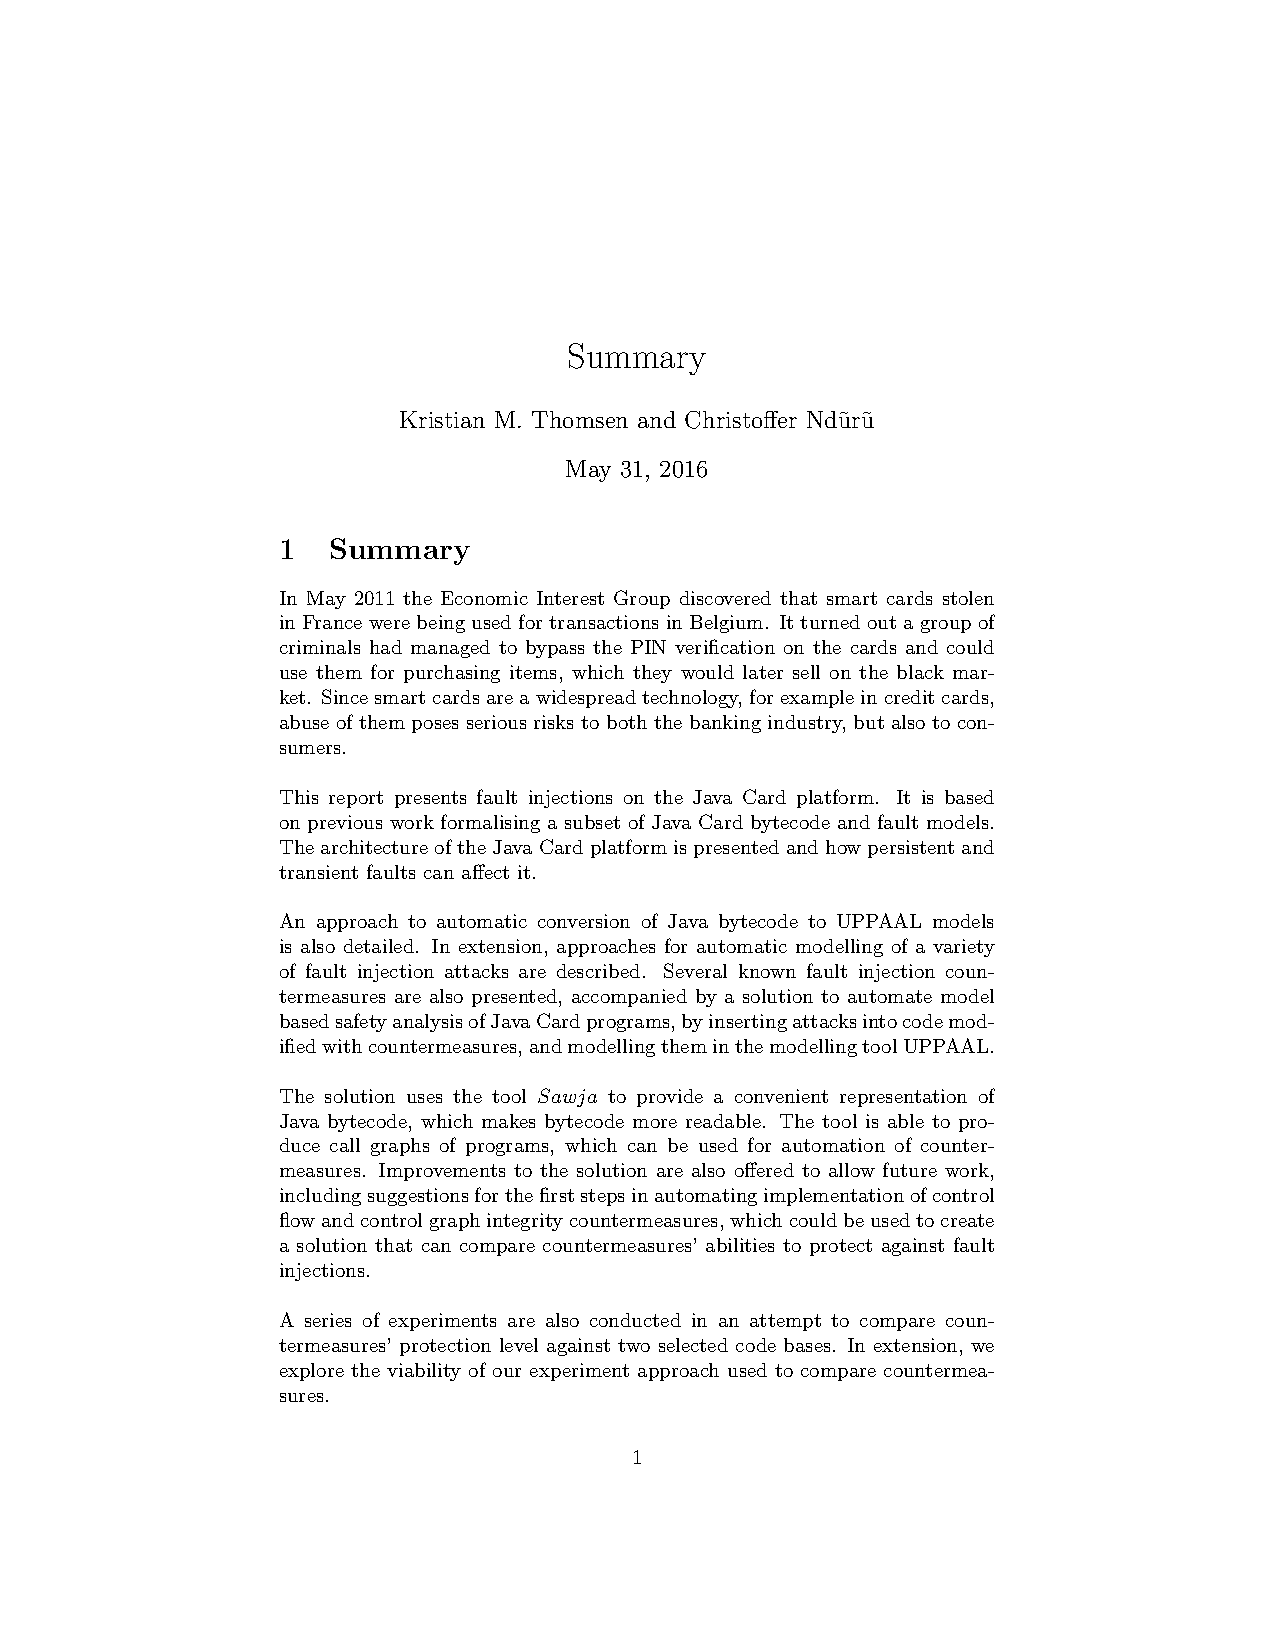
\includepdf[pages={1}]{documents/Front/summary/summary.pdf}
%!TEX root = ../../master.tex
\newcommand{\headerPreface}{Preface}
%\cleardoublepage
%\phantomsection
\pdfbookmark{\headerPreface}{chap:preface}
\chapter*{\headerPreface}\label{chap:preface}

%!TEX root = ../../master.tex
\newcommand{\headerPreface}{Preface}
%\cleardoublepage
%\phantomsection
\pdfbookmark{\headerPreface}{chap:preface}
\chapter*{\headerPreface}\label{chap:preface}

\input{documents/Introduction/preface}

\pagebreak
\subsubsection{Signatures}
\vspace{8ex}
\noindent\begin{tabular}{l}
\makebox[4in]{\hrulefill}\\
Christoffer Nd\~ur\~u\\[8ex]

\makebox[4in]{\hrulefill}\\
Kristian Mikkel Thomsen\\[8ex]
\end{tabular}

%\vspace{1em}

%We would like to thank our Supervisor Peter Dolog for his guidance and involvement in the project.
%Furthermore, we would like to thank the author of uClassify (a text classifier), Jon Kågström, for providing us with an Educational License to the server version of uClassify. 
%
%\vspace{1em}
%
%To the reader who is interested in the final product described by this report, we will host the application at \url{http://bit.ly/sw706e14} for as long as possible.
%Please note at the time being, it is not possible to associate a Facebook account without being added as a tester of the application.
%Also note that it is possible to register a user by supplying an email and password.

%%% Local Variables:
%%% mode: latex
%%% TeX-master: "../../master"
%%% End:


\pagebreak
\subsubsection{Signatures}
\vspace{8ex}
\noindent\begin{tabular}{l}
\makebox[4in]{\hrulefill}\\
Christoffer Nd\~ur\~u\\[8ex]

\makebox[4in]{\hrulefill}\\
Kristian Mikkel Thomsen\\[8ex]
\end{tabular}

%\vspace{1em}

%We would like to thank our Supervisor Peter Dolog for his guidance and involvement in the project.
%Furthermore, we would like to thank the author of uClassify (a text classifier), Jon Kågström, for providing us with an Educational License to the server version of uClassify. 
%
%\vspace{1em}
%
%To the reader who is interested in the final product described by this report, we will host the application at \url{http://bit.ly/sw706e14} for as long as possible.
%Please note at the time being, it is not possible to associate a Facebook account without being added as a tester of the application.
%Also note that it is possible to register a user by supplying an email and password.

%%% Local Variables:
%%% mode: latex
%%% TeX-master: "../../master"
%%% End:



% Some setup
%\setcounter{page}{4}
\setcounter{secnumdepth}{2}

\cleardoublepage
\phantomsection

%Table of content
\pdfbookmark{\contentsname}{toc}
\setcounter{tocdepth}{1}
\tableofcontents

\clearpage
%\afterpage{\null\newpage}
% Input contents
\cleardoublepage

\pagestyle{fancy}
\pagenumbering{arabic}

% Use include to do some latex magic when working on big reports
% Switches to temp .aux file to avoid recompilation of entire project
% Introduction

\chapter{Introduction}
% bite here
In May 2011 Economic Interest Group noticed that smart cards stolen in France were being used in Belgium\cite{fun}. It turned out a group of criminals, aided by an engineer, managed to perform a man-in-the middle attack on the credit cards by placing a chip on top of the original chip. The attack bypassed PIN verification by intercepting communication between a credit card terminal and the original chip. As a consequence, a transaction would be approved whether the correct PIN was entered on the terminal or not. The gang is estimated to have caused damages below \EUR{600,000}. They sold items purchased with the stolen cards on the black market, and managed to exploit over 7,000 transactions before being apprehended. Smart cards are found in many places today, everywhere from phone SIM cards in phones, access cards and credit cards. The first wide spread use was French pay phone cards in 1983\cite[p. 366]{modbank}.\\\\
% purpose of the report
This report shows that two selected attack countermeasures, code duplication and call graph integrity, improve the security of \jc bytecode. Several models of a program are presented and tested by simulation in the modelling tool UPPAAL\cite{uppaal_site} and its statistical model checking extension UPPAAL SMC\cite{uppaal_smc_site}, to assert that this is indeed true.
\kri{omskriv}
\chapter{Faults}\label{sec:faultsce}
\section{Fault Scenarios}\label{sec:faultsce}
We consider two general categories of faults that can occur to a \jc: \textit{persistent} and \textit{transient} faults. The main difference between these is that the persistent faults will affect the program every run, while the transient faults will only be present for a limited amount of time. Faults can occur when hardware is exposed to radiation sources, e.g. infrared light, laser, heat, physical abuse or cosmic radiation from space. 
% % %
Persistent faults in a piece of hardware, such as system memory, can occur in several way, suchas as a directed fault injection, e.g. a laser beam, targeting a persistent part of memory, such as the EEPROM of a \jc. This could cause a bit flip in a value that is persistent across power-ups, and thus cause a persistent fault since the wrong value will always be used. If one wishes to create a persistent fault, precision is important, both to strike a persistent part of memory, but also to affect the correct value.\\

% % %
% % % what about other ways?

% % %
Transient faults do not cause any permanent damage to the hardware. They can cause a temporary bit flip, resulting in a corrupted value, changed control flow to cause unintended behaviour, or a crash of the hardware. The altered behavior will disappear and the fault injection will have to be performed again, if the effect is to be reproduced.
% % %
Nonetheless, both persistent and transient faults can have fatal consequences, if they strike at the right time and the right place, e.g. for an attacker trying to change a programs control flow and thus execute a sensitive piece of code. 

The two categories of fault injection are thus sensitive to two variables, \textit{time} and \textit{place}, to different degrees. For example, an attacker who is trying to alter a constant in a program on a chipped access card, is able to work on the card in private surroundings. He can remove the protective layer on the chip and induce a persistent error on the card. Since the card is offline, the timing of the fault injection does not matter because he can only affect static values on the chip. The fault will still be present when the card is powered on at a later time. 

On the other hand, an attacker who wants to change transient properties such as program flow dependent on a non-constant value, is very dependent on both timing and precision of his attack. He has to affect the correct place in memory at just the right time in the program's execution to alter the program flow. \cref{tab:dependencies} illustrates the dependencies of persistent and transient fault injections.

\begin{table}[h!]
\centering
\begin{tabular}{|c|c|c|}
\hline  & Persistent & Transient \\ 
\hline Timing &  & X \\ 
\hline Precision & X & X \\ 
\hline 
\end{tabular} 
\caption{Table showing dependencies of induced faults}
\label{tab:dependencies}
\end{table}

% % which scenario have we chosen to focus on and why?
\christoffer{do we have to choose one or do we analyse both?}

It is important to note that when attacking the chip offline, the attacker only has access to persistently stored values. When attacking the card in online mode, the attacker also has access to run-time related values, such as user input values stored on the operand stack.\\\\
It is also interesting to note that an attacker performing a fault injection on the chip while it is offline, has to leave the card in an uncorrupted state, since it will not boot up correctly if e.g. the \textit{install()} method, described in~\cref{subsec:jcinstall}, of a \jc was hit by the fault injection, thus corrupting it. This is another reasion \textit{precision} is important. When performing a fault injection on a card which is online, the attacker can strike both persistent values and run-time values. The attacker additionally does not have to leave the card in an uncorrupted state as he would have to when injecting a fault on an offline card. The reason for this is that the attacker might only need to flip a particular bit in e.g. a response APDU packet, see \cref{subsec:apdu}, or an operand stack value, to trick a card terminal into accepting a transaction. After the card has sent the manipulated packet, the attacker does not care whether the card crashes since the purpose of the attack has been served.
\section{Fault Probabilities}
As mentioned in \Cref{sec:faultsce}, the time a bit flip is performed, matter in terms of how much of the system can be affected, e.g. at run-time versus when a card is powered off. Logically, a greater attack surface equals a greater probability of affecting a piece of memory that will cause a desirable outcome for an attacker. An example could be a method which is only runs once compared to a method which might be called ten times. Disregarding the size of the methods and their memory usage, the second method would have a probability ten times the that of the method which is only called once, to be hit by a bit flip. It should be noted that even if a method has a greater probability of being hit by a bit flip, it is not guarantee that there is a greater chance that the bit flip will bring the card into a situation compromising security. This depends on the nature of the method.


% install()
We have decided to not perform any simulation of bit flip attacks in the \texttt{install()} method, described in \cref{sec:jc}, and protection against these. The reason for this is, that for cards like credit cards, the method is only executed once and the execution happens at the manufacturer or distributor of the card.

%
\section{Java Card}\label{sec:jc}
\subsection{\texttt{install()}}
The \texttt{install()} method creates an instance of the \texttt{Applet} subclass\ch{ref to api docs page 65}. Depending on the application of the card, this method is called \textit{once} in a card's life time, from either the manufacturer's or card distributor's side. Examples of such cards are credit cards and SIM cards, since it could pose a security risk to allow other applets than those intended to be on the card, to be installed.\\\\
The install method should perform all necessary initialisations and must perform a call to the \texttt{register()} method. If the call to \texttt{register()} is not performed successfully, or an exception is thrown before the call, the installation is not considered successful. If the installation fails, the Java Card runtime environment performs the necessary clean up actions when control is returned to it. After a successful installation, the applet can be selected with the \texttt{select APDU} command.
\section{Related Work}\label{sub:faultCounter}
\subsection{Fault Injection}
\subsection{Countermeasures}\label{subsec:countermeasures}
\paragraph{Instruction Differentiation} 
A single bitflip can change the instruction being performed by changing the opcode of an instruction being executed, e.g. \texttt{ifeq} can be flipped to \texttt{ifne}, \texttt{iflt}, \texttt{ifgt} and \texttt{goto} in the \jc bytecode instruction set. This is particularly troublesome if the two instructions take the same number of parameters and put the same number of elements back on the operand stack. If this is the case, the operand stack will have the same number of elements on it whether the original or the altered instruction is executed, and the same number of parameters. It can therefore not be detected with e.g. a countermeasure such as Field of Bit, which detects a change in an instruction if the number of parameters change~\cite[p. 16]{javasec}\ch{fieldofbit usually implemented (source?)}.
%modification of the JVM instruction set binary representation
This can partly be remedied by modifying the underlying binary representations of the instructions in the Java Card Virtual Machine (JCVM)\ch{should this be generalised to just virtual machine since it is universally true for all virtual machines?}.
%fewer instructions with same parameter number and hamming distance 1
This would work by changing the representations in such a way that as few as possible instructions with the same number of parameters, and the same number of elements returned to the operand stack, are different by one bit. 
%not complete protection against bitflips, but improves misalignment detection rates
When a single bitflip changes an instruction, the chances that it is an undetectable change, in regards to required parameters and elements put back on the operand stack by it, are smaller than before modifying the representations.

%example table
\subsection{Code Duplication}as described by~\cite[p. 12]{javasec} is a countermeasure which protects against corruption of data used for branching at execution time, such as local variables. It offers protection against a change in a program's control flow, by duplicating instructions which are used to retrieve values which affect branching.\\\\
An example could be some original program, as the one in~\cref{lst:dup0}, which loads two values from local variables (line 1-2), pushes them onto the operand stack and compares them. If the two values are the same, a jump is performed to a code region with sensitive code (line 8-9), which approves a transaction on a credit card. Now, assume that a bit flip has occured in the flag set by the comparison in line 3. Before the flip, the rejection code would have been executed, but after the flip, the \texttt{acceptTransaction} is executed. When code duplication is implemented, as in~\cref{lst:dup1}, redundant instructions are inserted. In line 8-9, the values of the local variables are loaded again and pushed onto the operand stack. Afterwards, the compare flag is set again, and another jump is made to the sensitive code region in lines 15-16. It should be noted that this particular duplication only protects a \textit{single} bit flip in the original portion of the code. If a second bit flip occurs in the duplicated part of the code to affect the jump, the program can still execute \texttt{acceptTransaction}, even though it should not.

\begin{minipage}{\linewidth}
\begin{lstlisting}[caption={Original program without code duplication implemented. The code is written in \jcl. Note that for simplicity, the numbers in the left side are line numbers and do not denote the program counter values.}, label={lst:dup0}]
...
1: LOAD 1;
2: LOAD 2;
3: IF_CMPEQ 8;
<rejection code>
8: PUSH 0;
9: INVOKEVIRTUAL 12;  // acceptTransaction();
...
\end{lstlisting}
\end{minipage}

\begin{minipage}{\linewidth}
\begin{lstlisting}[caption={Modified program with code duplication implemented. The code is written in \jcl. Note that for simplicity, the numbers in the left side are line numbers and do not denote the program counter values.}, label={lst:dup1}]
...
1: LOAD 1;
2: LOAD 2;
3: IF_CMPEQ 8;
<rejection code>
8: LOAD 1;
9: LOAD 2;
10: IF_CMPEQ 15;
<bit flip detected code>
15: PUSH 0;
16: INVOKEVIRTUAL 12;  // acceptTransaction();
...
\end{lstlisting}
\end{minipage}

\paragraph{Call graph integrity} as described by~\cite[p. 12]{javasec}, is a countermeasure which attempts to detect changes in the call graph of a program, e.g. caused by a bit flip. The idea is to have a unique id set by every caller\ch{should examples include check from callee to caller?} before a call, which is checked by every callee to see if the call was made from a legal caller. This also works the other way around from callee to caller, where the the callee sets a unique id which is checked by the caller upon return.\\\\
In \cref{lst:dupCall0}, an example of the caller is shown. In line 5 the unique caller id is set and in line 6 it is loaded into a class variable containing the id of the current caller. In line 7 the method shown in \cref{lst:dupCall1}\ch{missing ref} is called. The caller id, 42, stored on the heap just before the method call, and the assigned id of the caller is already stored in another variable in memory are pushed onto the stack in line 1 of \ref{lst:dupCall1}\ch{missing ref}. They are then compared in line 2, and if the stored value is equal to the value set by the caller, the call graph integrity has been verified and the sensitive code beginning at line 8 is executed. Note that these examples do not show the callee setting a unique id to be verified upon return to the caller.

\begin{minipage}{\linewidth}
\begin{lstlisting}[caption={Caller with call graph integrity implemented. The code is written in \jcl. Note that for simplicity, the numbers in the left side are line numbers and do not denote the program counter values.}, label={lst:dupCall0}]
...
5: PUSH 42; 
6: PUT_STATIC 2;
7: INVOKE_STATIC 42;
...
\end{lstlisting}
\end{minipage}

\begin{minipage}{\linewidth}
\begin{lstlisting}[caption={Callee with call graph integrity implemented. The code is written in \jcl. Note that for simplicity, the numbers in the left side are line numbers and do not denote the program counter values.}, label={lst:dupCall0}]
1: GET_STATIC 2
2: GET_STATIC 3
3: IF_CMPEQ 8
4: <data corruption handling code>

// sensitive code region
8: ...
\end{lstlisting}
\end{minipage}
\section{Program Analysis with Sawja}\label{sec:sawja}
% intro about Sawja
We use the tool \textit{Sawja} (Static Analysis Workshop for JAva)~\cite{sawja} to analyse Java class files, and to create a call graph. Information from the graph can then be used to provide information for rewriting purposes, e.g. the call graph integrity countermeasure, described in \cref{sub:faultCounter}. Due to the \jc version of $Sawja$ not being public available, experiments are performed on Java code, but the principles remain the same.\\\\
% %
\cref{lst:javaorig} shows Java code where two classes are present, \texttt{A} and \texttt{B}. \texttt{B} inherits \texttt{A}, and both implement the method \texttt{bar()}. The implementation of the method that will be called depends on the boolean value \texttt{b}. When the compiled class file of this code is processed for a call graph by \textit{Sawja}, the result is as \cref{lst:callgraph} shows. The numbers that are listed just after the method calls, e.g. $40$ are interesting, since they cluster method call targets, which can not always be resolved statically. In our case, we can use this to see which methods the call graph integrity countermeasure should be implemented in. If a method is not called, \textit{Sawja} does not include it in the call graph.
% clustering of possible methods
In the case with code where it is impossible to tell which method will be called at run-time as in \cref{lst:javaorig}, \textit{Sawja} includes both, as in line 3 and 4.


\begin{lstlisting}[caption=Java sample.,language=Java,label=lst:javaorig]
public void foo(boolean b){
    (b ? new A() : new B()).bar();
}
\end{lstlisting}



\begin{lstlisting}[caption=Call graph generated by \textit{Sawja}.,language=Java,label=lst:callgraph]
void Sample.main(java.lang.String[]),22 -> void B.<init>()
void Sample.main(java.lang.String[]),12 -> void A.<init>()
void Sample.main(java.lang.String[]),40 -> short A.bar()
void Sample.main(java.lang.String[]),40 -> short B.bar()
\end{lstlisting}


\noindent It is also able to pretty print the bytecode so that it becomes easier to read as in \cref{lst:javasawja}. 
% inlining of constant pool
The tool also inlines the constant pool, as is evident in pc 7, 9, 12, 14 and 16. For example in pc 7, \texttt{new A} would normally be \texttt{new \#id} where the id would be a method reference stored with identifier \texttt{id} in the constant pool. This inlining makes for a more compact representation of the bytecode. Additionally, dead code does not show up in \textit{Sawja}'s output.
% line numbers
Note that in the output, the target of a \texttt{goto} is expressed in terms of a relative offset as seen in pc 11, and not a absolute program counter as in regular Java bytecode. The instruction in line 11 will jump to the instruction at program counter $21$.

\newpage
\begin{lstlisting}[caption=Sawja sample. Note that the numbers on the inner left side are program counter values.,numbers=none,language=Java,label=lst:javasawja]
public void foo ( bool 1 ) ;
		Concrete Method
    	Not parsed

0.  iload 1
1.  ifeq 13
4.  new A
7.  dup
8.  invokespecial void A.<init> ( )
        A.<init>
11. goto 10
14. new B
17. dup
18. invokespecial void B.<init> ( )
        B.<init>
21. invokevirtual short A.bar ( )
        B.bar
        A.bar
24. pop
25. return

\end{lstlisting}


\chapter{Rewriting a Java Program}
\section{Program Analysis with Sawja}\label{sec:sawja}
% intro about Sawja
We use the tool \textit{Sawja} (Static Analysis Workshop for JAva)~\cite{sawja} to analyse Java class files, and to create a call graph. Information from the graph can then be used to provide information for rewriting purposes, e.g. the call graph integrity countermeasure, described in \cref{sub:faultCounter}. Due to the \jc version of $Sawja$ not being public available, experiments are performed on Java code, but the principles remain the same.\\\\
% %
\cref{lst:javaorig} shows Java code where two classes are present, \texttt{A} and \texttt{B}. \texttt{B} inherits \texttt{A}, and both implement the method \texttt{bar()}. The implementation of the method that will be called depends on the boolean value \texttt{b}. When the compiled class file of this code is processed for a call graph by \textit{Sawja}, the result is as \cref{lst:callgraph} shows. The numbers that are listed just after the method calls, e.g. $40$ are interesting, since they cluster method call targets, which can not always be resolved statically. In our case, we can use this to see which methods the call graph integrity countermeasure should be implemented in. If a method is not called, \textit{Sawja} does not include it in the call graph.
% clustering of possible methods
In the case with code where it is impossible to tell which method will be called at run-time as in \cref{lst:javaorig}, \textit{Sawja} includes both, as in line 3 and 4.


\begin{lstlisting}[caption=Java sample.,language=Java,label=lst:javaorig]
public void foo(boolean b){
    (b ? new A() : new B()).bar();
}
\end{lstlisting}



\begin{lstlisting}[caption=Call graph generated by \textit{Sawja}.,language=Java,label=lst:callgraph]
void Sample.main(java.lang.String[]),22 -> void B.<init>()
void Sample.main(java.lang.String[]),12 -> void A.<init>()
void Sample.main(java.lang.String[]),40 -> short A.bar()
void Sample.main(java.lang.String[]),40 -> short B.bar()
\end{lstlisting}


\noindent It is also able to pretty print the bytecode so that it becomes easier to read as in \cref{lst:javasawja}. 
% inlining of constant pool
The tool also inlines the constant pool, as is evident in pc 7, 9, 12, 14 and 16. For example in pc 7, \texttt{new A} would normally be \texttt{new \#id} where the id would be a method reference stored with identifier \texttt{id} in the constant pool. This inlining makes for a more compact representation of the bytecode. Additionally, dead code does not show up in \textit{Sawja}'s output.
% line numbers
Note that in the output, the target of a \texttt{goto} is expressed in terms of a relative offset as seen in pc 11, and not a absolute program counter as in regular Java bytecode. The instruction in line 11 will jump to the instruction at program counter $21$.

\newpage
\begin{lstlisting}[caption=Sawja sample. Note that the numbers on the inner left side are program counter values.,numbers=none,language=Java,label=lst:javasawja]
public void foo ( bool 1 ) ;
		Concrete Method
    	Not parsed

0.  iload 1
1.  ifeq 13
4.  new A
7.  dup
8.  invokespecial void A.<init> ( )
        A.<init>
11. goto 10
14. new B
17. dup
18. invokespecial void B.<init> ( )
        B.<init>
21. invokevirtual short A.bar ( )
        B.bar
        A.bar
24. pop
25. return

\end{lstlisting}


\chapter{Semantics}\label{chap:semantics}
%!TEX root = ../../master.tex
In this chapter we describe and formalise the language \jcl, which contains a variation of the core instructions of the Java Card bytecode language. In this context the term core describes the basic set of instructions from which all other Java Card instructions can be built. 
We created this language because it is easier to model the fewer instructions in this language, rather than all the instructions in Java Card.
The full set of Java Card instructions can be built from combinations of the instructions in \jcl.
Furthermore, there exists no official formal semantics for the Java Card language.
The instructions of \jcl are defined as:
\begin{align*}
  Instructions = \{
  & \texttt{NOP}, && \texttt{PUSH } v, && \texttt{POP}, \\ 
  & \texttt{ADD}, && \texttt{DUP}, && \texttt{GOTO } a, \\ 
  & \texttt{IF\_CMPEQ } a, && \texttt{INVOKESTATIC } mid, && \texttt{RETURN},\\ 
  & \texttt{PUTSTATIC } fid, && \texttt{GETSTATIC } fid, && \texttt{LOAD } a, \\
  & \texttt{STORE } a, && \texttt{INVOKEVIRTUAL } mid, && \texttt{PUTFIELD } fid,\\ 
  & \texttt{GETFIELD } fid, && \texttt{NEW } ci && \}
\end{align*}

$\mathbb{N}$ is defined as the set of all natural numbers, including zero, and $\mathbb{Z}$ is defined as the set of all integers.
In the operational semantics we want to describe values as an integer between a minimum value and a maximum value, $Values = \{ x | x \in \mathbb{Z} \wedge x \geq \texttt{INT\_MIN} \wedge x \leq \texttt{INT\_MAX} \}$.
In addition we want a notion of addresses which is used to refer to an instruction in a method and mapping to the heap: $Addresses  = \mathbb{N}$.
A program counter is used to represent the current address $ProgramCounters = PC = Addresses$. Instructions with parameters, such as \texttt{PUSH } $v$, increment the program counter with more than one, since it uses more than one byte. \\

The program is a sequence of instructions, we denote a program as $P = (i_0, \ldots, i_k)$ where $k$ is the number of instructions in the program. 
A program consist solely of instructions $P \in Programs$ and $Programs =  \{ x | x \in Instructions^{*} \}$.
To access instructions we introduce a function accepting a program, method identifier, and a program counter. 
It returns the instruction in the method of the program at the program counter.
The function is defined as:
$$inst = Programs \times MethodID \times PC \to   Instructions$$
$$MethodID = \mathbb{N}$$

To describe a running program we use configurations.
A configuration is a 4-tuple consisting of a program, constant pool, heap and a call stack. 
$$Conf = Program \times ConstPool \times Heap \times CallStack$$
Executing an instruction means moving from one configuration to another. 
We will use $\vdash$ to indicate no change in the elements left of $\vdash$. 
For the semantic rules, no change will occur in program and constant pool e.g.:
$$CP, P \vdash \langle H, CS \rangle \rightarrow \langle H', CS' \rangle$$
Where $CP \in ConstPool$, $H,H' \in Heap$, and $CS, CS' \in CallStack$.
We use a shorthand dot notation to access elements of a tuple e.g. $conf.Program$ where $conf \in Conf$, indicates the program used in the configuration $conf$.\\

The heap can be described as a function which takes a heap address and returns either the address \textit{or} value associated with that address $Heap = Addresses \to   (Addresses + Values)_\perp$. $\perp$ represents an undefined value, and is included to describe that $Addresses$ can also map to undefined addresses/values in the heap.\\

The call stack is used to keep track of the current method scope, it is a sequence of stack frames $CallStack = StackFrames^{*}$.
A stack frame holds the method id, local variables, operand stack and the program counter for the method.

$$StackFrame = MethodID \times Locals \times OpStack \times PC $$

Local variables are represented by the function $Locals = \mathbb{N} \to   Values_\perp$. 
The operand stack is a sequence of values and addresses $OpStack = (Values + Addresses)^{*}$. \\

To represent objects we need classes in our language.
We represent classes as a 2-tuple with a possible super class and a function for resolving methods: $Class = Class_\perp \times Methods$.
$Class_\perp$ is the super class or $\perp$ in the case of no super class  
$Methods$ is the set of all method identifiers implemented by the class.
Object are represented by a 2-tuple with the class and fields of the object: 
$$Object = Class \times Fields$$ 

Fields is a function for resolving the values of class variables:
$$Fields = FieldID \mapsto (Values + Addresses)$$ 
$$FieldID = \mathbb{N}$$

Finally we make use of a constant pool to resolve static method ids, fields of static classes and class definition when creating new objects:
$$CP = ConstPool = (MethodID \to \mathbb{N}) + (FieldID \to Addresses) + (ClassIndex \to  Class)$$
$$ClassIndex = \mathbb{N}$$

%%% Local Variables:
%%% mode: latex
%%% TeX-master: "../../master"
%%% End:

\section{Instruction Semantics}
In the following semantics we make use of these abbreviation:
\begin{subequations}
\begin{align*}
H, H' &\in Heap  & CS &\in CallStack & ops, ops', ops'' &\in OpStack\\
mid, mid', mid'' &\in MethodID & loc, loc' &\in Locals & pc, pc' &\in PC\\
v &\in Values & a, objr &\in Addresses & fid &\in FieldID \\
obj, obj' &\in Object & cl &\in Class
\end{align*}
\end{subequations}
%!TEX root = ../../master.tex


\subsection{NOP}
%This instruction has no effect other than incremented $PC$ by one.
The instruction has no other effect than incrementing the $pc$.
%The no operation (NOP) instruction does nothing. Therefore only the program counter, $PC$, is incremented to point to the next instruction to be executed. Additionaly, it should also be checked whether the instruction we are currently executing is indeed a NOP. This is done with $inst(P, mid, pc) = \texttt{NOP}$\\

%This results in a changed program counter, but an unchanged stack. The operational semantics for the NOP instruction are then as follows:
%$$\inference[NOP]{PC' = PC + 1 \semsp inst(P, PC) = \texttt{NOP}}{CP, P \vdash \langle PC, S \rangle \Rightarrow \langle PC', S \rangle}$$\\

$$\inference[NOP]{inst(P, mid, pc) = \texttt{NOP}}
% % % % % % % % % % % % % % % %
{CP, P \vdash \langle H, (CS, \langle mid, loc, ops, pc \rangle)\rangle \Rightarrow 
 \langle H, (CS, \langle mid, loc, ops, pc + 1 \rangle)\rangle
}$$

%{CP, P \vdash \langle PC, S \rangle \Rightarrow \langle PC', S \rangle}$$\\

%%% Local Variables:
%%% mode: latex
%%% TeX-master: "../../master"
%%% End:

\subsection{PUSH}
\texttt{PUSH} $v$ is used to add the value from the parameter $v$ onto the top of the operand stack. Since the \texttt{PUSH} $v$ instruction takes up two bytes due to the parameter, $pc$ is incremented by two.
$$\inference[PUSH]{
inst(P, mid, pc) = \texttt{PUSH }v \semnl\\
 ops = (x_0,\ldots,x_n) \semsp ops' = (x_0, \ldots, x_n, v) \ }
{CP, P \vdash \langle H, (CS, \langle mid, loc, ops, pc \rangle)\rangle \Rightarrow
 \langle H, (CS, \langle mid, loc, ops', pc + 2 \rangle)\rangle}$$\\

\subsection{POP}
This will remove and discard the top element of the operand stack.

$$\inference[POP]{
inst(P, mid, pc) = \texttt{POP} \semnl \\
ops = (x_0, \ldots, x_{n-1}, x_n) \semsp 
ops' = (x_0, \ldots, x_{n-1})}
{CP, P \vdash \langle H, (CS, \langle mid, loc, ops, pc \rangle)\rangle  \Rightarrow \langle H, (CS, \langle mid, loc, ops', pc + 1 \rangle)\rangle}$$

\subsection{ADD}
$$\inference[ADD]{ 
inst(P, mid, pc) = \texttt{ADD} \semsp
v = x_{k-1} + x_k \semnl \\
ops = (x_0,x_1, \ldots,x_{k-2},x_{k-1},x_k)\semsp
ops' = (x_0 \ldots x_{k-2},v)
}
{CP, P \vdash H, (CS, \langle mid, loc, ops, pc \rangle) \Rightarrow 
 H, (CS, \langle mid, loc, ops', pc + 1 \rangle)
}$$


\subsection{DUP}
\texttt{DUP} duplicates the top element of the operand stack, leaving two identical elements as the two top elements of the operand stack.
$$\inference[DUP]{ 
inst(P, mid, pc) = \texttt{DUP} \semnl \\
ops = (x_0, \ldots,x_n)\semsp
ops' = (x_0, \ldots, x_{n}, x_{n})
}
{CP, P \vdash \langle H, (CS, \langle mid, loc, ops, pc \rangle)\rangle \Rightarrow \langle H, (CS, \langle mid, loc, ops', pc + 1 \rangle)\rangle
}$$


%!TEX root = ../../master.tex
\subsection{GOTO}
\texttt{GOTO} $a$ takes an address as parameter and performs a jump to the specified address.

$$\inference[GOTO]{
inst(P, mid, pc) = \texttt{GOTO } a \semsp
pc' = a}
{CP, P \vdash \langle H, (CS, \langle mid, loc, ops, pc \rangle)\rangle \Rightarrow \langle H, (CS, \langle mid, loc, ops, pc' \rangle)\rangle}$$

%%% Local Variables:
%%% mode: latex
%%% TeX-master: "../../master"
%%% End:

%!TEX root = ../../master.tex
\subsection{IF\_CMPEQ}
This compares and consumes the two top elements of the operand stack.
If they are equal it will make a jump to the address given as a parameter, otherwise it will increment $pc$ by two.

$$inst(P, mid, pc) = \texttt{IF\_CMPEQ }a$$
\[
    pc'= 
\begin{cases}
    a,& \text{if } x_{n-1} = x_n\\
    pc+2,              & \text{otherwise}
\end{cases}
\]
$$\inference[IF\_CMPEQ]{ops=(x_0, \ldots, x_{n-2}, x_{n-1}, x_n) \semsp ops'=(x_0, \ldots, x_{n-2})}
{CP, P \vdash \langle H, (CS, \langle mid, locals, ops, pc \rangle)\rangle \Rightarrow \langle H, (CS, \langle mid, locals, ops', pc' \rangle)\rangle}$$

%!TEX root = ../../master.tex
\subsection{INVOKESTATIC}
\texttt{INVOKESTATIC} $mid$ is used to call a static method.
%This involves adding a new stack frame on the call stack with  locals which are the parameters taken by the method being the parameters taken by the method as well as local variables.
This involves adding a new stack frame on the call stack.
The parameters of the methods are stored in local variables of that stack frame.
These parameters are read from the operand stack.
The number of parameters, $pn$, are found in the constant pool. 

$$\inference[INVOKESTATIC]{
inst(P,mid,pc) = \texttt{INVOKESTATIC }mid' \semsp 
CP(mid') = pn \semnl \\
ops = (x_0, \ldots, x_n) \semsp
ops' = (x_0, \ldots, x_{n-pn}) \semnl\\
loc' = [0 \mapsto x_{n-pn}, \ldots, pn \mapsto x_n])}
{CP, P \vdash \langle H, (CS, \langle mid, loc, ops, pc \rangle)\rangle \Rightarrow }$$
$$\langle H, (CS, \langle mid, loc, ops', pc \rangle, \langle mid', loc', \epsilon, 0 \rangle)\rangle$$
%%% Local Variables:
%%% mode: latex
%%% TeX-master: "../../master"
%%% End:

\subsection{RETURN}
\texttt{RETURN} is used when returning from a method.
The result of a \texttt{RETURN} depends on the state of the operand stack when called.
If the operand stack is not empty the top element will be the return value.

$$\inference[RETURN]{
inst(P,mid',pc') = \texttt{RETURN} \semsp
ops = (x_0, \ldots, x_n) \semnl \\
ops' \neq \epsilon \semsp
ops' = (x'_0, \ldots, x'_n) \semsp
ops'' = (x_0, \ldots, x_n, x'_n)} 
{CP, P \vdash \langle H, (CS, \langle mid, loc, ops, pc \rangle, \langle mid', loc', ops', pc' \rangle)\rangle \Rightarrow}$$
$$ \langle H, (CS, \langle mid, loc, ops'', pc + 1 \rangle)\rangle$$

In following case, where the operand stack is empty, it will return without adding an element to the previous frame's operand stack.

$$\inference[RETURN VOID]{
inst(P,mid',pc') = \texttt{RETURN} \semsp
ops' = \epsilon }
{CP, P \vdash \langle H, (CS, \langle mid, loc, ops, pc \rangle, \langle mid', loc', ops', pc' \rangle)\rangle \Rightarrow}$$
$$ \langle H, (CS, \langle mid, loc, ops, pc + 1 \rangle)\rangle$$
%%% Local Variables:
%%% mode: latex
%%% TeX-master: "../../master"
%%% End:

\subsection{PUTSTATIC}
This is used to write a value to a class variable on the heap.

$$\inference[PUTSTATIC]{
inst(P,mid, pc) = \texttt{PUTSTATIC } fid \semnl \\
CP(fid) = a\semsp
H' = H[a\mapsto v] \semnl \\
ops = (x_0, \ldots, x_n, v) \semsp 
ops' = (x_0, \ldots, x_{n})
}
{CP, P \vdash \langle H, (CS, \langle mid, loc, ops, pc \rangle )\rangle \Rightarrow \langle H', (CS, \langle mid, loc, ops', pc + 2 \rangle )\rangle}$$
%%% Local Variables:
%%% mode: latex
%%% TeX-master: "../../master"
%%% End:

\subsection{GETSTATIC}
This reads the value of a class variable on the heap.

$$\inference[GETSTATIC]{  
inst(P, mid, pc) = \texttt{GETSTATIC }fid\semnl \\
CP(fid) = a \semsp 
H(a) = v \semsp 
v \neq \perp \semnl \\
ops = (x_0, \ldots, x_n) \semsp 
ops' = (x_0, \ldots, x_n, v) 
}
{CP, P \vdash \langle H, (CS, \langle  mid, loc, ops, pc \rangle)\rangle \Rightarrow \langle H, (CS, \langle mid, loc, ops', pc+2 \rangle)\rangle}$$

%%% Local Variables:
%%% mode: plain-tex
%%% TeX-master: "../../master"
%%% End:

\subsection{LOAD}
\texttt{LOAD} $i$ is used to load the value of a local variable onto the operand stack.

$$\inference[LOAD]{
inst(P, mid, pc) = \texttt{LOAD } i \semsp 
loc(i) = v \semsp
v \neq \perp \semnl \\
ops = (x_0 \ldots x_n) \semsp
ops' = (x_0 \ldots x_n,v)  
}
{CP, P \vdash \langle H, (CS, \langle mid, loc, ops, pc \rangle)\rangle \Rightarrow 
 \langle H, (CS, \langle mid, loc, ops', pc + 2 \rangle)\rangle 
}$$

%%% Local Variables:
%%% mode: latex
%%% TeX-master: "../../master"
%%% End:

%!TEX root = ../../master.tex
\subsection{STORE}
This will store a new value in a local variable.

$$\inference[STORE]{
inst(P,mid, pc) = \texttt{STORE }i \semsp
loc' = loc[i \mapsto x_n]\semnl\\
ops = (x_0, \ldots, x_{n-1}, x_n) \semsp 
ops' = (x_0, \ldots, x_{n-1})
}
{CP, P \vdash \langle H, (CS, \langle mid, loc, ops, pc \rangle )\rangle \Rightarrow \langle H, (CS, \langle mid, loc', ops', pc + 2 \rangle )\rangle}$$

%!TEX root = ../../master.tex
\subsection{INVOKE\_VIRTUAL}
\texttt{INVOKEVIRTUAL} is similar to \texttt{INVOKESTATIC} but in addition an object reference from the operand stack is stored as the first local variable, and the method for the actual class is resolved by a method lookup, inspired by \cite{dalvik}. For this we introduce two functions $signa$, and $methodLookup$. $signa = MethodID \to Signature$, where $Signature$ is the method's signature e.g. name and parameters. And $methodLookup$ used to lookup the intended method identifier, either from the class itself or a super class, defined as: \\\\
$methodLookup(mid, cl) = $ \vspace{-10px}
\[
\begin{cases}
  \perp & if\ cl = \perp \\
  mid'  & if\ mid' \in cl.Methods \wedge signa(mid') = signa (mid)  \\
  methodLookup(mid, cl.Class) & otherwise
\end{cases}
\]


$$\inference[INVOKEVIRTUAL]{
inst(P,mid,pc) = \texttt{INVOKEVIRTUAL }mid' \semsp 
CP(mid') = pn \semnl \\
ops = (x_0, \ldots, x_n, objr, p_1, \ldots, p_{pn}) \semsp
ops' = (x_0, \ldots, x_{n}) \semnl\\ 
methodLookup(H(objr).Class, mid') = mid'' \semsp
mid'' \neq \perp \semnl\\
loc' = [0 \mapsto objr, 1 \mapsto p_{1}, \ldots, pn \mapsto p_{pn}]
}
{CP, P \vdash \langle H, (CS, \langle mid, loc, ops, pc \rangle)\rangle \Rightarrow }$$
$$\hspace{130px}\langle H, (CS, \langle mid, loc, ops', pc \rangle, \langle mid'', loc', \epsilon, 0 \rangle)\rangle$$
\kristian{private vs public calls}
%%% Local Variables:
%%% mode: latex
%%% TeX-master: "../../master"
%%% End:

%!TEX root = ../../master.tex
\subsection{PUT\_FIELD}
\texttt{PUTFIELD} $fid$ takes an object reference and a value from the top of the operand stack and stores the value in a specific field in the object.

$$\inference[PUTFIELD]{
inst(P,mid, pc) = \texttt{PUTFIELD } fid \semsp
H(objr) = obj \semnl \\
H' = H[objr \mapsto obj'] \semsp 
obj' = obj.Fields[fid \mapsto v] \semnl\\
ops = (x_0, \ldots, x_n, objr, v) \semsp
ops' = (x_0, \ldots, x_{n})}
{CP, P \vdash \langle H, (CS, \langle mid, loc, ops, pc \rangle )\rangle \Rightarrow \langle H', (CS, \langle mid, loc, ops', pc + 2 \rangle )\rangle}$$
\subsection{GETFIELD}
\texttt{GETFIELD} $fid$ reads and consumes an object reference from the operand stack, and reads the value of the specified field in the object which is then stored on the operand stack. 

$$\inference[GETFIELD]{
inst(P,mid, pc) = \texttt{GETFIELD }fid \semnl\\
obj = H(objr) \semsp
v = obj.Fields(fid)\semnl \\
ops = (x_0, \ldots, x_n, objr) \semsp ops' = (x_0, \ldots, x_n, v)}
{CP, P \vdash \langle H, (CS, \langle mid, loc, ops, pc \rangle )\rangle \Rightarrow \langle H, (CS, \langle mid, loc, ops', pc + 2 \rangle )\rangle}$$

%!TEX root = ../../master.tex
\subsection{NEW}
\texttt{NEW} $ci$ creates a new object on the heap as well as pushing an object reference to the operand stack.

$$\inference[NEW]{
inst(P,mid, pc) = \texttt{NEW }ci \semsp
CP(ci) = cl \semnl \\
obj = \langle cl, fields \rangle \semsp
fields \in Fields \semnl \\
H(objr) = \perp \semsp
H' = H[objr \mapsto obj]  \semnl \\
ops = (x_0, \ldots, x_n) \semsp
ops' = (x_o, \ldots, x_n, objr)
}
{CP, P \vdash \langle H, (CS, \langle mid, loc, ops, pc \rangle )\rangle \Rightarrow \langle H', (CS, \langle mid, loc, ops', pc + 2 \rangle )\rangle}$$
%%% Local Variables:
%%% mode: latex
%%% TeX-master: "../../master"
%%% End:


%!TEX root = ../../master.tex
\section{Fault Semantics}

\chapter{UPPAAL and Formal Verification}
\section{Property Verification}
UPPALL has its own query language used to verify properties of a model\cite[p. 7]{upptut}. The language is a simplified version of timed computation tree logic. UPPAAL's query language consists of \textit{state formulae} and \textit{path formulae}. The path formulae can be categorised into three categories: reachability, safety and liveness. These are described below, and they are summarised in \cref{fig:query}.
\paragraph{State formulae}
A state formula is an expression which can be evaluated for a state, without looking at the mode, e.g. $i \geq 42$. This formula asks whether it is true that $i$ is greater than or equal to $42$ in a given state. State formulae also allow one to verify whether a process is in a given location using an expression of the form \texttt{P.l}, where \texttt{P} is a process and \texttt{l} is a location in the process.\\\\
%deadlock special case
A deadlock is described using a special state formula, \texttt{deadlock}, and is satisfied for all states which deadlock.
\paragraph{Reachability properties} express the notion that a state formula, $\varphi$, can \textit{possibly} be satisfied on some path, going from the initial location of the model. In UPPAAL it is expressed as \texttt{E<>$\varphi$}. This could for example be used to verify whether a variable \texttt{i} in the model, along some path going from the initial location will have the value $2$ by querying the model with \texttt{E<>i == 2}.\\\\
These types of properties are often verified as a part of a sanity check of a modelled system\cite[p. 8]{upptut}, e.g. that it is possible to reach the done location in a \jc program. Though this does not give any guarantee that the program will always finish, it makes sense to make sure to check whether it \textit{possibly} can.
\paragraph{Safety properties} state that ``something bad will never happen''. In other words, every state in a model will invariantly satisfy $\varphi$. This is useful e.g. to check that a bit flip can not cause a modelled program to end up in a location where e.g. incorrect credentials are authenticated and subsequently approved. Such an invariant safety property is expressed in UPPAAL as \texttt{A[]$\varphi$}, where the state formula, $\varphi$, would express that the simulation of the model would never end up in the approved location when the credentials are incorrect.\\\\
A variant of this safety property, is one that expresses that ``something will possibly never happen'', e.g. when playing a game, a safe state would be one where a winning move is always possible. This is expressed in UPPAAL as \texttt{E[]$\varphi$}, which states that there should exist a maximal path\footnote{A maximal path, is a path that is either infinite or the last state has no outgoing edges that can be traversed.}, where $\varphi$ is always true.
\paragraph{Liveness property} state that ``something will eventually happen'', e.g. verify that the program will eventually reach the end location. It is expressed in UPPAAL as \texttt{A<>$\varphi$}, and means that $\varphi$ is eventually satisfied.\\\\
A variation of this liveness property, is the \textit{leads to} property, written as $\varphi \leadsto \psi$. It is expressed in a UPPAAL query as \texttt{$\varphi$ --> $\psi$}, and means that if $\varphi$ is satisfied, $\psi$ will eventually be satisfied, e.g. when \jc transaction is begun, it will eventually end\footnote{A transaction in respect to \jc, is a number of instructions which should be executed atomically.}.

\begin{figure}[H]
\centering
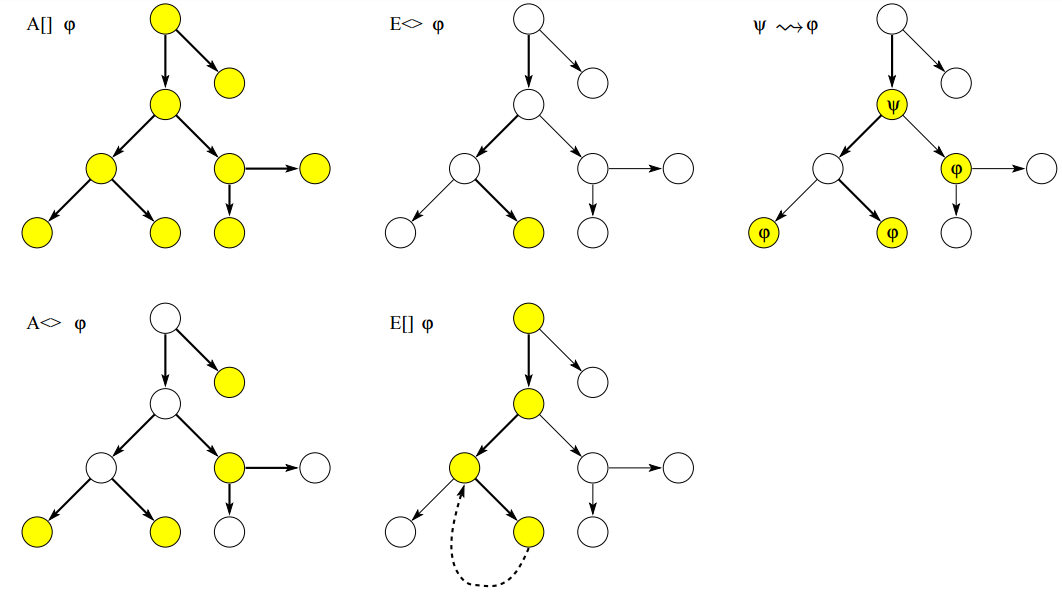
\includegraphics[width=0.9\textwidth]{queries.png}
\caption{Illustration of the different property verification queries in UPPAAL. Taken from \cite[p. 8]{upptut}}.
\label{fig:query}
\end{figure}

\section{SMC}
extra edges for waiting
\chapter{Building a UPPAAL Model}
\section{Program Representation}
When translating a program to a UPPAAL of the program. Several representations are possible, depending on what one wants to show. One could for example represent a program merely in terms of program flow if a simulation of a disruption of the program flow is to be shown, e.g an error in the program counter. One could also include the data flow in the program if a simulation of a corruption of a memory value is to be shown. These are just a few examples and many representations can be chosen.\\

We have chosen the later and model the program in terms of program flow and data flow, so that we can simulation disruptions in the programs execution flow. 


\subsection{Representation Details}
The program simulation is based on \jcl semantics, most Java bytecodes can be translated directly to \jcl at the loss of type information.\\
\kri{what does it mean for us?}
When representing Java bytecode in UPPAAL we have chosen to represent an instruction, such as \texttt{aload a} and \texttt{dup}, as UPPAAL locations. 
This implies that a change in the program counter is a change of the location. 
In turn this means that when an instruction is to be executed the change to the program configuration \textit{Conf} from  \cref{sec:semintro} occurs on the edge to next location.

\begin{lstlisting}[caption=Jave code sample.]
public class Sample{
    public static void main(String[] args) {
        for (String a : args)         
        {
            System.out.print(a);
        }
    }
}
\end{lstlisting}

\begin{lstlisting}[caption=Bytecode sample.]
public static void main(java.lang.String[]);
 Code:
   0: aload_0       
   1: astore_1      
   2: aload_1       
   3: arraylength   
   4: istore_2      
   5: iconst_0      
   6: istore_3      
   7: iload_3       
   8: iload_2       
   9: if_icmpge     31
  12: aload_1       
  13: iload_3       
  14: aaload        
  15: astore        4
  17: getstatic     #2                  // Field java/lang/System.out:Ljava/io/PrintStream;
  20: aload         4
  22: invokevirtual #3                  // Method java/io/PrintStream.print:(Ljava/lang/String;)V
  25: iinc          3, 1
  28: goto          7
  31: return        

\end{lstlisting}

\begin{figure}[H]
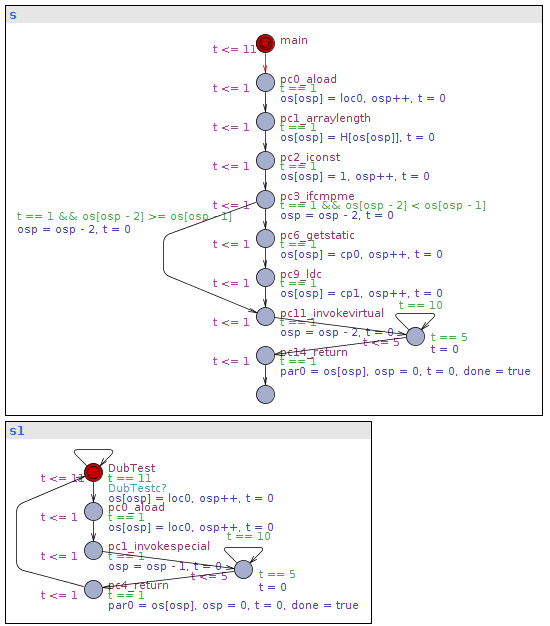
\includegraphics[width=\textwidth]{generated_wip}
\caption{Auto generated model, work in progress.}
\label{fig:generated_wip}
\end{figure}
\kri{update the model for the new sample}

\subsubsection{Simple Instructions}
\begin{figure}[H]
\centering
\begin{subfigure}{.3\textwidth}
  \begin{lstlisting}
  0. aload 0
  1. arraylength
  ...
  \end{lstlisting}
  \caption{Java Bytecode Sample.}
\end{subfigure} 
\hspace{10px}
\begin{subfigure}{.6\textwidth}
  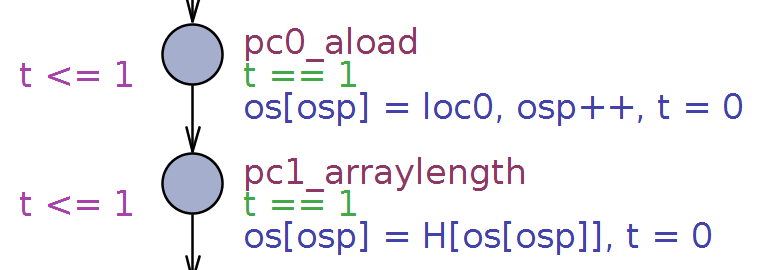
\includegraphics[width=\textwidth]{UPPAAL1.png}
  \caption{Generated model from Sample.}
\end{subfigure}
\caption{Java bytecode and corresponding UPPAAL model.}
\label{fig:uppaal1}
\end{figure}
\kri{lav ny model til nyt sample}
\Cref{fig:uppaal1} show how two Java Bytecode instructions are represented in UPPAAL. On the left we see the Java bytecode, the first line with program counter 0 we have the \texttt{aload 0} instruction. \texttt{aload 0} pushes a reference to the top of the operation stack from local variables at position zero, then increments the operand stack pointer and program counter.

%uppaal location edge
In UPPAAL the location \texttt{pc0\_aload} represent \texttt{aload 0}. The UPPAAL model is seen in \Cref{fig:uppaal1}b. We simulate execution time with the location invariant \texttt{t <= 1}  and guard \texttt{t == 1} on the edge leading to the next location. The guard is found right below the location name right of the edge and invariant is to the left of the edge. In this sample we defined the execution time as 1 time unit.

In the update on the edge seen below the guard, we simulate the data flow by assigning the value of the local variable \texttt{loc0} to the top of the operand stack \texttt{os} represented by operand stack pointer \texttt{osp}. \texttt{osp} is incremented as the operand stack grows, the increment of the program counter is simulated by the edge itself.

\subsubsection{Jumps and Branches}
For the majority of instructions the program counter is set to the next instruction after execution, but for a jump with \texttt{goto a} the edge goes to the instruction with the program counter corresponding with value of \texttt{a}.

Conditionals such as \texttt{if\_cmpeq a} is the only instruction that is modelled by a location having two outgoing edges , one to the next instruction and one for the program counter of a. On these edges the guard is used to determine which of the edges is to be traversed. \kri{insert example}
\subsubsection{Method Calls}\label{subsubsec:method}
Method calls are represented by three additions to the model. These additions consist of locations, but they do not have any associated program counter since they are not a part of the original program.\\

% special case for main
The first is an addition of a location in the template of the \texttt{main} method. This location captures the notion that this is the start of the program.\\

% caller
The second is a new location in the caller for every method call it performs. This makes it possible to simulate parameter passing, as well as control transfer when waiting for a callee to return control to the caller after a method call. The simulation of the caller remains in this location until the callee returns control, after its simulation has finished. This control transfer is modeled with a synchronisation on the edge going from the new state in the caller and back to its original control flow.\ch{insert ref to figure}~\\

% callee
The third is an addition of two additional states in every template, except for the \texttt{main} template. The first, initial, location serves dual purposes: it enables the control transfer from the caller to itself by synchronisation, and simulates passing of arguments into the method from the caller. The second location is the \textit{Done} location, where the simulation ends up when it has finished its simulation. This is where control is transferred back to the caller.
\ch{show how parameters are passed in figure}
\ch{rewrite this}
\section{Modelling a Fault Injection}
To simulate a single bit flip occurring in the program's execution a special fault template is introduced. The template calculates a random value between $0$ and the maximum possible global clock value, which represents when in the programs execution a fault happens. The random value is assigned to a global variable in the UPPAAL system.\\\\
Every instruction in the Java bytecode is represented by a location, and has an associated program counter. There are edges from each location going to the locations which can be reached if one bit is flipped in the program counter. These edges have guards which check whether the time the fault is injected, corresponds to the global clock at the time the model simulation is at that particular edge. If it is, the guard will allow the edge to be traversed. There are no fault edges going back to the added locations described in \cref{subsubsec:method}, since these are not a part of the original program and therefore do not have an associated program counter.
\begin{figure}[H]
\centering
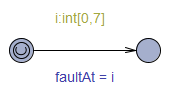
\includegraphics{figures/fault.PNG}
\caption{The UPPAAL template which performs a bit flip in the program counter}
\end{figure}\ch{update figure to use fault at between 0 and global clock}


\subsection{Opstack complications}
Under normal execution the value of the operand stack pointer can be known at compile  time \kri{double check, etv find source}. This leaves us with two ways to simulate it, use a operand stack pointer to point at the top element or staticly define the opstack element to be accessed for each instruction.

Under normal execution there is to difference between the two approaches, but then introducing fault models as PC\_Fault and INST\_Fault it is possible to change the behaviour. This can let the operand stack pointer point to a value an instruction never would access or in the extreme case go out of bounds for the method.

Our approach is the operand stack pointer and assume that the virtual machine will detect out of bounds. As such under a PC\_FAULT a former value of might be read instead of the current one.

The Java Virtual Machine assumes that ``There are no operand stack overflows or underflows'' \cite[c. 4.10]{java_specc} which is checked by the verifier.

\chapter{Experiments}


Opstack pointer assumption is broken\\\\
Inst fault og Instruction Differentiation\\\\
Code dub\\\\
Call graph integrity\\\\

\chapter{Conclusion}
\section{Future Work}


% Appendices
\appendix
\numberwithin{figure}{chapter}
\numberwithin{table}{chapter}
\chapter{Sample Model}
\begin{figure}
  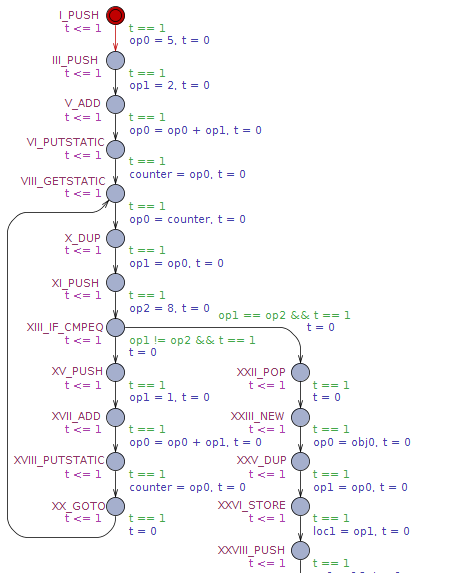
\includegraphics[width=\textwidth]{timed1.png}
  \caption{Model of full \jcl}
\end{figure}
\begin{figure}
  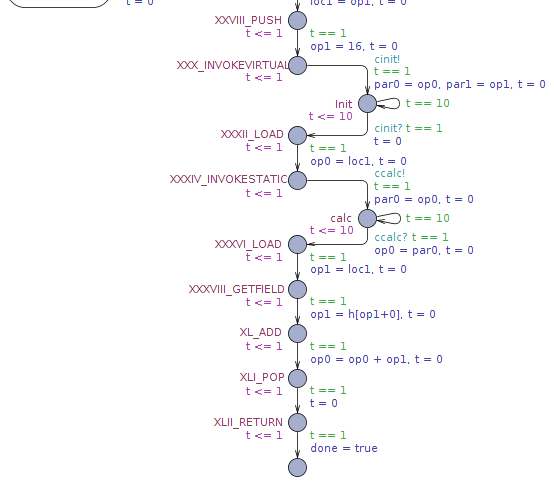
\includegraphics[width=\textwidth]{timed2.png}
  \caption{Model of full \jcl}
\end{figure}
\begin{figure}
  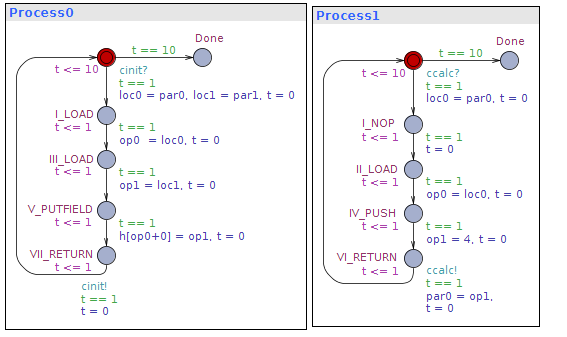
\includegraphics[width=\textwidth]{timed3.png}
  \caption{Model of full \jcl}
\end{figure}

\chapter{Semantics}\label{chap:semantics}
%!TEX root = ../../master.tex
In this chapter we describe and formalise the language \jcl, which contains a variation of the core instructions of the Java Card bytecode language. In this context the term core describes the basic set of instructions from which all other Java Card instructions can be built. 
We created this language because it is easier to model the fewer instructions in this language, rather than all the instructions in Java Card.
The full set of Java Card instructions can be built from combinations of the instructions in \jcl.
Furthermore, there exists no official formal semantics for the Java Card language.
The instructions of \jcl are defined as:
\begin{align*}
  Instructions = \{
  & \texttt{NOP}, && \texttt{PUSH } v, && \texttt{POP}, \\ 
  & \texttt{ADD}, && \texttt{DUP}, && \texttt{GOTO } a, \\ 
  & \texttt{IF\_CMPEQ } a, && \texttt{INVOKESTATIC } mid, && \texttt{RETURN},\\ 
  & \texttt{PUTSTATIC } fid, && \texttt{GETSTATIC } fid, && \texttt{LOAD } a, \\
  & \texttt{STORE } a, && \texttt{INVOKEVIRTUAL } mid, && \texttt{PUTFIELD } fid,\\ 
  & \texttt{GETFIELD } fid, && \texttt{NEW } ci && \}
\end{align*}

$\mathbb{N}$ is defined as the set of all natural numbers, including zero, and $\mathbb{Z}$ is defined as the set of all integers.
In the operational semantics we want to describe values as an integer between a minimum value and a maximum value, $Values = \{ x | x \in \mathbb{Z} \wedge x \geq \texttt{INT\_MIN} \wedge x \leq \texttt{INT\_MAX} \}$.
In addition we want a notion of addresses which is used to refer to an instruction in a method and mapping to the heap: $Addresses  = \mathbb{N}$.
A program counter is used to represent the current address $ProgramCounters = PC = Addresses$. Instructions with parameters, such as \texttt{PUSH } $v$, increment the program counter with more than one, since it uses more than one byte. \\

The program is a sequence of instructions, we denote a program as $P = (i_0, \ldots, i_k)$ where $k$ is the number of instructions in the program. 
A program consist solely of instructions $P \in Programs$ and $Programs =  \{ x | x \in Instructions^{*} \}$.
To access instructions we introduce a function accepting a program, method identifier, and a program counter. 
It returns the instruction in the method of the program at the program counter.
The function is defined as:
$$inst = Programs \times MethodID \times PC \to   Instructions$$
$$MethodID = \mathbb{N}$$

To describe a running program we use configurations.
A configuration is a 4-tuple consisting of a program, constant pool, heap and a call stack. 
$$Conf = Program \times ConstPool \times Heap \times CallStack$$
Executing an instruction means moving from one configuration to another. 
We will use $\vdash$ to indicate no change in the elements left of $\vdash$. 
For the semantic rules, no change will occur in program and constant pool e.g.:
$$CP, P \vdash \langle H, CS \rangle \rightarrow \langle H', CS' \rangle$$
Where $CP \in ConstPool$, $H,H' \in Heap$, and $CS, CS' \in CallStack$.
We use a shorthand dot notation to access elements of a tuple e.g. $conf.Program$ where $conf \in Conf$, indicates the program used in the configuration $conf$.\\

The heap can be described as a function which takes a heap address and returns either the address \textit{or} value associated with that address $Heap = Addresses \to   (Addresses + Values)_\perp$. $\perp$ represents an undefined value, and is included to describe that $Addresses$ can also map to undefined addresses/values in the heap.\\

The call stack is used to keep track of the current method scope, it is a sequence of stack frames $CallStack = StackFrames^{*}$.
A stack frame holds the method id, local variables, operand stack and the program counter for the method.

$$StackFrame = MethodID \times Locals \times OpStack \times PC $$

Local variables are represented by the function $Locals = \mathbb{N} \to   Values_\perp$. 
The operand stack is a sequence of values and addresses $OpStack = (Values + Addresses)^{*}$. \\

To represent objects we need classes in our language.
We represent classes as a 2-tuple with a possible super class and a function for resolving methods: $Class = Class_\perp \times Methods$.
$Class_\perp$ is the super class or $\perp$ in the case of no super class  
$Methods$ is the set of all method identifiers implemented by the class.
Object are represented by a 2-tuple with the class and fields of the object: 
$$Object = Class \times Fields$$ 

Fields is a function for resolving the values of class variables:
$$Fields = FieldID \mapsto (Values + Addresses)$$ 
$$FieldID = \mathbb{N}$$

Finally we make use of a constant pool to resolve static method ids, fields of static classes and class definition when creating new objects:
$$CP = ConstPool = (MethodID \to \mathbb{N}) + (FieldID \to Addresses) + (ClassIndex \to  Class)$$
$$ClassIndex = \mathbb{N}$$

%%% Local Variables:
%%% mode: latex
%%% TeX-master: "../../master"
%%% End:

\section{Instruction Semantics}
In the following semantics we make use of these abbreviation:
\begin{subequations}
\begin{align*}
H, H' &\in Heap  & CS &\in CallStack & ops, ops', ops'' &\in OpStack\\
mid, mid', mid'' &\in MethodID & loc, loc' &\in Locals & pc, pc' &\in PC\\
v &\in Values & a, objr &\in Addresses & fid &\in FieldID \\
obj, obj' &\in Object & cl &\in Class
\end{align*}
\end{subequations}
%!TEX root = ../../master.tex


\subsection{NOP}
%This instruction has no effect other than incremented $PC$ by one.
The instruction has no other effect than incrementing the $pc$.
%The no operation (NOP) instruction does nothing. Therefore only the program counter, $PC$, is incremented to point to the next instruction to be executed. Additionaly, it should also be checked whether the instruction we are currently executing is indeed a NOP. This is done with $inst(P, mid, pc) = \texttt{NOP}$\\

%This results in a changed program counter, but an unchanged stack. The operational semantics for the NOP instruction are then as follows:
%$$\inference[NOP]{PC' = PC + 1 \semsp inst(P, PC) = \texttt{NOP}}{CP, P \vdash \langle PC, S \rangle \Rightarrow \langle PC', S \rangle}$$\\

$$\inference[NOP]{inst(P, mid, pc) = \texttt{NOP}}
% % % % % % % % % % % % % % % %
{CP, P \vdash \langle H, (CS, \langle mid, loc, ops, pc \rangle)\rangle \Rightarrow 
 \langle H, (CS, \langle mid, loc, ops, pc + 1 \rangle)\rangle
}$$

%{CP, P \vdash \langle PC, S \rangle \Rightarrow \langle PC', S \rangle}$$\\

%%% Local Variables:
%%% mode: latex
%%% TeX-master: "../../master"
%%% End:

\subsection{PUSH}
\texttt{PUSH} $v$ is used to add the value from the parameter $v$ onto the top of the operand stack. Since the \texttt{PUSH} $v$ instruction takes up two bytes due to the parameter, $pc$ is incremented by two.
$$\inference[PUSH]{
inst(P, mid, pc) = \texttt{PUSH }v \semnl\\
 ops = (x_0,\ldots,x_n) \semsp ops' = (x_0, \ldots, x_n, v) \ }
{CP, P \vdash \langle H, (CS, \langle mid, loc, ops, pc \rangle)\rangle \Rightarrow
 \langle H, (CS, \langle mid, loc, ops', pc + 2 \rangle)\rangle}$$\\

\subsection{POP}
This will remove and discard the top element of the operand stack.

$$\inference[POP]{
inst(P, mid, pc) = \texttt{POP} \semnl \\
ops = (x_0, \ldots, x_{n-1}, x_n) \semsp 
ops' = (x_0, \ldots, x_{n-1})}
{CP, P \vdash \langle H, (CS, \langle mid, loc, ops, pc \rangle)\rangle  \Rightarrow \langle H, (CS, \langle mid, loc, ops', pc + 1 \rangle)\rangle}$$

\subsection{ADD}
$$\inference[ADD]{ 
inst(P, mid, pc) = \texttt{ADD} \semsp
v = x_{k-1} + x_k \semnl \\
ops = (x_0,x_1, \ldots,x_{k-2},x_{k-1},x_k)\semsp
ops' = (x_0 \ldots x_{k-2},v)
}
{CP, P \vdash H, (CS, \langle mid, loc, ops, pc \rangle) \Rightarrow 
 H, (CS, \langle mid, loc, ops', pc + 1 \rangle)
}$$


\subsection{DUP}
\texttt{DUP} duplicates the top element of the operand stack, leaving two identical elements as the two top elements of the operand stack.
$$\inference[DUP]{ 
inst(P, mid, pc) = \texttt{DUP} \semnl \\
ops = (x_0, \ldots,x_n)\semsp
ops' = (x_0, \ldots, x_{n}, x_{n})
}
{CP, P \vdash \langle H, (CS, \langle mid, loc, ops, pc \rangle)\rangle \Rightarrow \langle H, (CS, \langle mid, loc, ops', pc + 1 \rangle)\rangle
}$$


%!TEX root = ../../master.tex
\subsection{GOTO}
\texttt{GOTO} $a$ takes an address as parameter and performs a jump to the specified address.

$$\inference[GOTO]{
inst(P, mid, pc) = \texttt{GOTO } a \semsp
pc' = a}
{CP, P \vdash \langle H, (CS, \langle mid, loc, ops, pc \rangle)\rangle \Rightarrow \langle H, (CS, \langle mid, loc, ops, pc' \rangle)\rangle}$$

%%% Local Variables:
%%% mode: latex
%%% TeX-master: "../../master"
%%% End:

%!TEX root = ../../master.tex
\subsection{IF\_CMPEQ}
This compares and consumes the two top elements of the operand stack.
If they are equal it will make a jump to the address given as a parameter, otherwise it will increment $pc$ by two.

$$inst(P, mid, pc) = \texttt{IF\_CMPEQ }a$$
\[
    pc'= 
\begin{cases}
    a,& \text{if } x_{n-1} = x_n\\
    pc+2,              & \text{otherwise}
\end{cases}
\]
$$\inference[IF\_CMPEQ]{ops=(x_0, \ldots, x_{n-2}, x_{n-1}, x_n) \semsp ops'=(x_0, \ldots, x_{n-2})}
{CP, P \vdash \langle H, (CS, \langle mid, locals, ops, pc \rangle)\rangle \Rightarrow \langle H, (CS, \langle mid, locals, ops', pc' \rangle)\rangle}$$

%!TEX root = ../../master.tex
\subsection{INVOKESTATIC}
\texttt{INVOKESTATIC} $mid$ is used to call a static method.
%This involves adding a new stack frame on the call stack with  locals which are the parameters taken by the method being the parameters taken by the method as well as local variables.
This involves adding a new stack frame on the call stack.
The parameters of the methods are stored in local variables of that stack frame.
These parameters are read from the operand stack.
The number of parameters, $pn$, are found in the constant pool. 

$$\inference[INVOKESTATIC]{
inst(P,mid,pc) = \texttt{INVOKESTATIC }mid' \semsp 
CP(mid') = pn \semnl \\
ops = (x_0, \ldots, x_n) \semsp
ops' = (x_0, \ldots, x_{n-pn}) \semnl\\
loc' = [0 \mapsto x_{n-pn}, \ldots, pn \mapsto x_n])}
{CP, P \vdash \langle H, (CS, \langle mid, loc, ops, pc \rangle)\rangle \Rightarrow }$$
$$\langle H, (CS, \langle mid, loc, ops', pc \rangle, \langle mid', loc', \epsilon, 0 \rangle)\rangle$$
%%% Local Variables:
%%% mode: latex
%%% TeX-master: "../../master"
%%% End:

\subsection{RETURN}
\texttt{RETURN} is used when returning from a method.
The result of a \texttt{RETURN} depends on the state of the operand stack when called.
If the operand stack is not empty the top element will be the return value.

$$\inference[RETURN]{
inst(P,mid',pc') = \texttt{RETURN} \semsp
ops = (x_0, \ldots, x_n) \semnl \\
ops' \neq \epsilon \semsp
ops' = (x'_0, \ldots, x'_n) \semsp
ops'' = (x_0, \ldots, x_n, x'_n)} 
{CP, P \vdash \langle H, (CS, \langle mid, loc, ops, pc \rangle, \langle mid', loc', ops', pc' \rangle)\rangle \Rightarrow}$$
$$ \langle H, (CS, \langle mid, loc, ops'', pc + 1 \rangle)\rangle$$

In following case, where the operand stack is empty, it will return without adding an element to the previous frame's operand stack.

$$\inference[RETURN VOID]{
inst(P,mid',pc') = \texttt{RETURN} \semsp
ops' = \epsilon }
{CP, P \vdash \langle H, (CS, \langle mid, loc, ops, pc \rangle, \langle mid', loc', ops', pc' \rangle)\rangle \Rightarrow}$$
$$ \langle H, (CS, \langle mid, loc, ops, pc + 1 \rangle)\rangle$$
%%% Local Variables:
%%% mode: latex
%%% TeX-master: "../../master"
%%% End:

\subsection{PUTSTATIC}
This is used to write a value to a class variable on the heap.

$$\inference[PUTSTATIC]{
inst(P,mid, pc) = \texttt{PUTSTATIC } fid \semnl \\
CP(fid) = a\semsp
H' = H[a\mapsto v] \semnl \\
ops = (x_0, \ldots, x_n, v) \semsp 
ops' = (x_0, \ldots, x_{n})
}
{CP, P \vdash \langle H, (CS, \langle mid, loc, ops, pc \rangle )\rangle \Rightarrow \langle H', (CS, \langle mid, loc, ops', pc + 2 \rangle )\rangle}$$
%%% Local Variables:
%%% mode: latex
%%% TeX-master: "../../master"
%%% End:

\subsection{GETSTATIC}
This reads the value of a class variable on the heap.

$$\inference[GETSTATIC]{  
inst(P, mid, pc) = \texttt{GETSTATIC }fid\semnl \\
CP(fid) = a \semsp 
H(a) = v \semsp 
v \neq \perp \semnl \\
ops = (x_0, \ldots, x_n) \semsp 
ops' = (x_0, \ldots, x_n, v) 
}
{CP, P \vdash \langle H, (CS, \langle  mid, loc, ops, pc \rangle)\rangle \Rightarrow \langle H, (CS, \langle mid, loc, ops', pc+2 \rangle)\rangle}$$

%%% Local Variables:
%%% mode: plain-tex
%%% TeX-master: "../../master"
%%% End:

\subsection{LOAD}
\texttt{LOAD} $i$ is used to load the value of a local variable onto the operand stack.

$$\inference[LOAD]{
inst(P, mid, pc) = \texttt{LOAD } i \semsp 
loc(i) = v \semsp
v \neq \perp \semnl \\
ops = (x_0 \ldots x_n) \semsp
ops' = (x_0 \ldots x_n,v)  
}
{CP, P \vdash \langle H, (CS, \langle mid, loc, ops, pc \rangle)\rangle \Rightarrow 
 \langle H, (CS, \langle mid, loc, ops', pc + 2 \rangle)\rangle 
}$$

%%% Local Variables:
%%% mode: latex
%%% TeX-master: "../../master"
%%% End:

%!TEX root = ../../master.tex
\subsection{STORE}
This will store a new value in a local variable.

$$\inference[STORE]{
inst(P,mid, pc) = \texttt{STORE }i \semsp
loc' = loc[i \mapsto x_n]\semnl\\
ops = (x_0, \ldots, x_{n-1}, x_n) \semsp 
ops' = (x_0, \ldots, x_{n-1})
}
{CP, P \vdash \langle H, (CS, \langle mid, loc, ops, pc \rangle )\rangle \Rightarrow \langle H, (CS, \langle mid, loc', ops', pc + 2 \rangle )\rangle}$$

%!TEX root = ../../master.tex
\subsection{INVOKE\_VIRTUAL}
\texttt{INVOKEVIRTUAL} is similar to \texttt{INVOKESTATIC} but in addition an object reference from the operand stack is stored as the first local variable, and the method for the actual class is resolved by a method lookup, inspired by \cite{dalvik}. For this we introduce two functions $signa$, and $methodLookup$. $signa = MethodID \to Signature$, where $Signature$ is the method's signature e.g. name and parameters. And $methodLookup$ used to lookup the intended method identifier, either from the class itself or a super class, defined as: \\\\
$methodLookup(mid, cl) = $ \vspace{-10px}
\[
\begin{cases}
  \perp & if\ cl = \perp \\
  mid'  & if\ mid' \in cl.Methods \wedge signa(mid') = signa (mid)  \\
  methodLookup(mid, cl.Class) & otherwise
\end{cases}
\]


$$\inference[INVOKEVIRTUAL]{
inst(P,mid,pc) = \texttt{INVOKEVIRTUAL }mid' \semsp 
CP(mid') = pn \semnl \\
ops = (x_0, \ldots, x_n, objr, p_1, \ldots, p_{pn}) \semsp
ops' = (x_0, \ldots, x_{n}) \semnl\\ 
methodLookup(H(objr).Class, mid') = mid'' \semsp
mid'' \neq \perp \semnl\\
loc' = [0 \mapsto objr, 1 \mapsto p_{1}, \ldots, pn \mapsto p_{pn}]
}
{CP, P \vdash \langle H, (CS, \langle mid, loc, ops, pc \rangle)\rangle \Rightarrow }$$
$$\hspace{130px}\langle H, (CS, \langle mid, loc, ops', pc \rangle, \langle mid'', loc', \epsilon, 0 \rangle)\rangle$$
\kristian{private vs public calls}
%%% Local Variables:
%%% mode: latex
%%% TeX-master: "../../master"
%%% End:

%!TEX root = ../../master.tex
\subsection{PUT\_FIELD}
\texttt{PUTFIELD} $fid$ takes an object reference and a value from the top of the operand stack and stores the value in a specific field in the object.

$$\inference[PUTFIELD]{
inst(P,mid, pc) = \texttt{PUTFIELD } fid \semsp
H(objr) = obj \semnl \\
H' = H[objr \mapsto obj'] \semsp 
obj' = obj.Fields[fid \mapsto v] \semnl\\
ops = (x_0, \ldots, x_n, objr, v) \semsp
ops' = (x_0, \ldots, x_{n})}
{CP, P \vdash \langle H, (CS, \langle mid, loc, ops, pc \rangle )\rangle \Rightarrow \langle H', (CS, \langle mid, loc, ops', pc + 2 \rangle )\rangle}$$
\subsection{GETFIELD}
\texttt{GETFIELD} $fid$ reads and consumes an object reference from the operand stack, and reads the value of the specified field in the object which is then stored on the operand stack. 

$$\inference[GETFIELD]{
inst(P,mid, pc) = \texttt{GETFIELD }fid \semnl\\
obj = H(objr) \semsp
v = obj.Fields(fid)\semnl \\
ops = (x_0, \ldots, x_n, objr) \semsp ops' = (x_0, \ldots, x_n, v)}
{CP, P \vdash \langle H, (CS, \langle mid, loc, ops, pc \rangle )\rangle \Rightarrow \langle H, (CS, \langle mid, loc, ops', pc + 2 \rangle )\rangle}$$

%!TEX root = ../../master.tex
\subsection{NEW}
\texttt{NEW} $ci$ creates a new object on the heap as well as pushing an object reference to the operand stack.

$$\inference[NEW]{
inst(P,mid, pc) = \texttt{NEW }ci \semsp
CP(ci) = cl \semnl \\
obj = \langle cl, fields \rangle \semsp
fields \in Fields \semnl \\
H(objr) = \perp \semsp
H' = H[objr \mapsto obj]  \semnl \\
ops = (x_0, \ldots, x_n) \semsp
ops' = (x_o, \ldots, x_n, objr)
}
{CP, P \vdash \langle H, (CS, \langle mid, loc, ops, pc \rangle )\rangle \Rightarrow \langle H', (CS, \langle mid, loc, ops', pc + 2 \rangle )\rangle}$$
%%% Local Variables:
%%% mode: latex
%%% TeX-master: "../../master"
%%% End:


%!TEX root = ../../master.tex
\section{Fault Semantics}


\chapter{Code Samples}
\label{chap:samples}
\begin{lstlisting}[caption={Mocked Java example code from the Java Card samples},label={lst:example}]
// Example.java
public class Example 
{
    public static void main(String[] args) {
        try
        {
		  Example hw = new Example();
        }catch (Exception ex)
        {

        }
    }

    public Example() throws Exception
    {
        processVerifyPIN();
    }

    private void processVerifyPIN() throws Exception
    {
        int pinLength = 4;
        int faultCode = 255;
        int triesRemaining;

        short count = setIncomingAndReceive();    // get expected data

        if(count < pinLength) throw new Exception();

        if(isInvalid() != false)
        {
            triesRemaining = getTriesRemaining();
            throw new Exception();
        }
    }


    private boolean isInvalid()
    {
        return true;
    }

    private short setIncomingAndReceive()
    {
        return 5;
    }

    private int getTriesRemaining()
    {
        return 2;
    }
}
\end{lstlisting}

\newpage

\begin{lstlisting}[caption={Mocked Java example code from the Java Card samples with the call graph integrity countermeasure implemented},label={lst:exampleCGI}]
// ExampleCGI.java
public class ExampleCGI
{
    private static int callId;

    public static void main(String[] args) {
        try
        {
            callId = 1;
		    ExampleCGI hw = new ExampleCGI();

        if(!(callId == 2))
        {
            throw new Exception();
        }

        }catch (Exception ex)
        {

        }
    }

    public ExampleCGI() throws Exception
    {
        if(callId != 1)
        {
            throw new Exception();
        }

        callId = 2;

        processVerifyPIN();

        if(callId != 3)
        {
            throw new Exception();
        }

        callId = 2;
    }

    private void processVerifyPIN() throws Exception
    {
        if(callId != 2)
        {
            throw new Exception();
        }

        int pinLength = 4;
        int faultCode = 255;
        int triesRemaining;

        callId = 3;

        short count = setIncomingAndReceive();    // get expected data

        if(callId != 4)
        {
            throw new Exception();
        }

        if(count < pinLength) throw new Exception();

        callId = 4;

        if(isInvalid() != false)
        {
            if(callId != 5)
            {
                throw new Exception();
            }

            callId = 5;
            triesRemaining = getTriesRemaining();
            
            if(callId != 6)
            {
                throw new Exception();
            }

            throw new Exception();
        }

        callId = 2;
    }


    private boolean isInvalid() throws Exception
    {
        if(callId != 4)
        {
            throw new Exception();
        }

        callId = 5;

        return true;
    }

    private short setIncomingAndReceive() throws Exception
    {
        if(callId != 3)
        {
            throw new Exception();
        }

        callId = 4;
        return 5;
    }

    private int getTriesRemaining() throws Exception
    {
        if(callId != 5)
        {
            throw new Exception();
        }

        callId = 6;

        return 2;
    }
}
\end{lstlisting}

\begin{lstlisting}[caption={Java bytecode example of the code duplication countermeasure},label={lst:exampleBytecode}]
Class Example

private bool  isInvalid ();  
Concrete Method
Parsed     

Example.processVerifyPIN()    
0.  iconst 1
1.  ireturn

 public  Example ();  Concrete Method   Parsed      Example.main(java.lang.String[])    
0.  aload  0
1.  invokespecial  void  java.lang.Object.<init> ()
4.  aload  0
5.  invokespecial  void  Example.processVerifyPIN ()
8.  return

 private void  processVerifyPIN ();  Concrete Method   Parsed      Example.<init>()    
0.  iconst 4
1.  istore  1
2.  sipush 255
5.  istore  2
6.  aload  0
7.  invokespecial  short  Example.setIncomingAndReceive ()
10.  istore  4
12.  iload  4
14.  iload  1
15.  ifcmpge 11
18.  new  java.lang.Exception
21.  dup
22.  invokespecial  void  java.lang.Exception.<init> ()
25.  athrow
26.  aload  0
27.  invokespecial  bool  Example.isInvalid ()
30.  ifeq 16
33.  aload  0
34.  invokespecial  int  Example.getTriesRemaining ()
37.  istore  3
38.  new  java.lang.Exception
41.  dup
42.  invokespecial  void  java.lang.Exception.<init> ()
45.  athrow
46.  aload  0
47.  invokespecial  bool  Example.isInvalid ()
50.  ifeq 4
53.  goto -20
54.  return

 public static void  main ( java.lang.String [] 0);  Concrete Method   Parsed  
0.  new  Example
3.  dup
4.  invokespecial  void  Example.<init> ()
7.  astore  1
8.  goto 4
11.  astore  1
12.  return

try start: 0; try end: 8: catch start: 11; catched type: java.lang.Exception.

private int  getTriesRemaining (); 
Concrete Method   
Parsed      

Example.processVerifyPIN()    
0.  iconst 2
1.  ireturn

private short  setIncomingAndReceive ();  Concrete Method   Parsed      Example.processVerifyPIN()    
0.  iconst 5
1.  ireturn

\end{lstlisting}

\begin{lstlisting}[caption={Java code example of the control flow integrity countermeasure},label={lst:examplecfi}]

public class ExampleCFI
{
	private static int flag = 0;
	
    public static void main(String[] args) {
        try
        {
		  ExampleCFI hw = new ExampleCFI();
        }catch (Exception ex)
        {

        }
    }

    public ExampleCFI() throws Exception
    {
        processVerifyPIN();
		
		if(flag != 3)
		{
			throw new Exception();
		}
    }

    private void processVerifyPIN() throws Exception
    {
		flag++;
		
        int pinLength = 4;
        int faultCode = 255;
        int triesRemaining;

        short count = setIncomingAndReceive();    // get expected data
		
        if(count < pinLength) throw new Exception();

        if(isInvalid() != false)
        {
            triesRemaining = getTriesRemaining();
            throw new Exception();
        }
    }


    private boolean isInvalid()
    {
		flag++;
        return true;
    }

    private short setIncomingAndReceive()
    {
		flag++;
        return 5;
    }

    private int getTriesRemaining()
    {
        return 2;
    }


}
\end{lstlisting}
\ch{fix indents in code}

\label{totalpage}

% Bibliography
\label{biblo}
\bibliography{sources}

%Count the last page	
\label{lastpage}
\end{document}

%%% Local Variables:
%%% mode: latex
%%% TeX-master: t
%%% End:
